\typeout{ ====================================================================}
\typeout{ this is file main.tex, created at 20 Nov 2012                       }
\typeout{ maintained by Gustavo Rabello dos Anjos                             }
\typeout{ e-mail: gustavo.rabello@gmail.com                                   }
\typeout{ ====================================================================}

\documentclass[a4paper,fleqn,12pt,twoside]{report} % tipo de folha e documento
\usepackage[T1]{fontenc}              % acentuacao e hifenizacao portuguesa
%\usepackage[utf8]{inputenc}
\usepackage[brazil]{babel}            % pacote de linguagens 
\usepackage{indentfirst}              % tab na primeira linha do paragrafo 
\usepackage[hmargin=30mm,vmargin=25mm]{geometry}
\usepackage{graphicx}         % pacote para inclusao de figuras,
\usepackage{subfig,wrapfig}           % pacote para figuras duplas (subfigure)
\usepackage{amssymb,amsmath,amsfonts} % pacote matematicos
\usepackage{multirow}                 % multiplas linhas por coluna
\usepackage{pictexwd,color}			  % ambiente para PICTEX
\usepackage{tocbibind}				  % para inclusao de bib e ind na TOC
\usepackage{alltt,verbatim,moreverb}  % para entrada verbatim comandos LaTeX
\usepackage{rotating}				  % para rotacionar alguns flutuantes
\usepackage{amscd}					  % para setas longas

\graphicspath{{./figs/}{./figs.eps/}}  % onde encontrar as figuras...

\renewcommand{\baselinestretch}{1.5}  % espacamento entre linhas 
\setlength{\mathindent}{15mm}         % espacamento das equacoes

%%%%%%%%%%%%%%%%%%%%%%%%%%%%%%%%  MATH MACROS %%%%%%%%%%%%%%%%%%%%%%%%%%%%%%%%
\newcommand{\tr}{{\,\rm tr}\,}
\newcommand{\sen}{{\,\rm sen}\,}
\newcommand{\senh}{{\,\rm senh}\,}
\newcommand{\diverg}{{\,\rm div}\,}
\newcommand{\grad}{\,\mathbf{grad}\,}
\newcommand{\rot}{\,\mathbf{rot}\,}
\newcommand{\uvet}{\mathbf{u}}
\newcommand{\vvet}{\mathbf{v}}
\newcommand{\wvet}{\mathbf{w}}
\newcommand{\xvet}{\mathbf{x}}
\newcommand{\gvet}{\mathbf{g}}
\newcommand{\fvet}{\mathbf{f}}
\newcommand{\nvet}{\mathbf{n}}
\newcommand{\tvet}{\mathbf{t}}
\newcommand{\Imat}{\mathbf{I}}
\newcommand{\Eo}{\mathrm{Eo}}
\newcommand{\N}{\mathrm{N}}
\newcommand{\Mo}{\mathrm{Mo}}
%%%%%%%%%%%%%%%%%%%%%%%%%%%%%%%%%  -- END -- %%%%%%%%%%%%%%%%%%%%%%%%%%%%%%%%%

\begin{document}

%--------------------------------------------------
% \noindent Gustavo Anjos \\
% \noindent
% \textsl{Nuclear Science and Engineering
% \\
% \noindent MIT -- Massachusetts Institute of Technology}
%-------------------------------------------------- 
 
\chapter{Introdu\c c\~ao aos Escoamentos Bif\'asicos}

A proposta deste cap\'itulo \'e dar ao leitor uma vis\~ao geral dos
m\'etodos mais importantes encontrados na literatura de escoamentos
bif\'asicos. Uma revis\~ao  bibliogr\'afica \'e tamb\'em inclu\'ida para
ajudar o leitor a encontrar as principais refer\^encias e nomes de
autores que desenvolveram metodologias para a investiga\c c\~ao deste
importante fen\^omeno.

\section{Introdu\c c\~ao}

Os escoamentos bif\'asicos s\~ao encontrados abundantemente na natureza.
A presen\c ca de fluidos que n\~ao se misturam pode ser notada em todo
tipo de aplica\c c\~ao, desde o contato do oceano com a atmosf\'era,
at\'e centrais de produ\c c\~ao e extra\c c\~ao de petr\'oleo, onde o
\'oleo se encontra a altas temperaturas com a presen\c ca de bolhas de
g\'as. O conceito de fase, atrav\'es dos princ\'ipios de termodin\^amica
cl\'assica, \'e descrito como o estado macrosc\'opico da mat\'eria no
qual sua estrutura f\'isica e sua composi\c c\~ao qu\'imica s\~ao
homog\^eneas. Na presen\c ca de duas ou mais fases, origina-se o que
chamamos de escoamentos multif\'asicos, onde o termo bif\'asico se
refere \`a presen\c ca de apenas 2 fases (Ex. bolha de g\'as carb\^onico
em um copo de \'agua gaseificada).

A Fig.~(\ref{fig:surfTension}) exemplifica em forma esquem\'atica,
algumas situa\c c\~oes decorrentes da riqueza e complexidade do
fen\^onemno bif\'asico e que muitas vezes nos passa desapercebido. No
primeiro exemplo (Fig.~(\ref{fig:surfTension}a) podemos observar a
presen\c ca de uma for\c ca capaz de equilibrar a esfera sobre a coluna
de l\'iquido. Para o caso representado, onde o somat\'orio das for\c cas
\'e nulo, a grandeza respons\'avel pela sustenta\c c\~ao da esfera se
chama tens\~ao superficial. Este efeito f\'isico aparece na camada
superficial do l\'iquido e age como uma membrana el\'astica. A tens\~ao
superficial depende do sistema bif\'asico e pode variar conforme as
propriedades f\'isicas dos fluidos, a temperatura ou, ainda, com a
contamina\c c\~ao dos fluidos. O segundo exemplo
(Fig.~(\ref{fig:surfTension}b) representa o fen\^omeno de capilaridade
ou a\c c\~ao capilar, que \'e a capacidade do fluido de vencer os
efeitos gravitacionais e subir sobre as paredes dos tubos. Um exemplo
pode ser facilmente notado em um copo de \'agua onde se verifica um
abaulamento do l\'iquido junto \`a superf\'icie do copo. No terceiro
exemplo (Fig.~(\ref{fig:surfTension}c)) e no quarto exemplo
(Fig.~(\ref{fig:surfTension}d)) s\~ao ilustradas duas gotas em repouso. Na
figura pode-se observar que o contato do l\'iquido com uma superf\'icie
s\'olida pode variar a forma da gota. Esta diferen\c ca de forma \'e
atribuida ao tipo de superf\'ice em contato com o fluido. As
superf\'icies hidrof\'ilicas tendem a permitir um espalhamento do
l\'iquido enquanto que as superf\'icies hidrof\'obicas fazem com que a
gota se mantenha concentrada na superf\'icie. Num caso extremo,
conhecido como superf\'icies super hidrof\'obicas, a \'area da gota em
contato com a superf\'icie \'e m\'inima, mantendo a gota em sua forma
esf\'erica. 


\begin{figure}[h!]
	\begin{center}
		\subfloat[esfera em repouso]
		{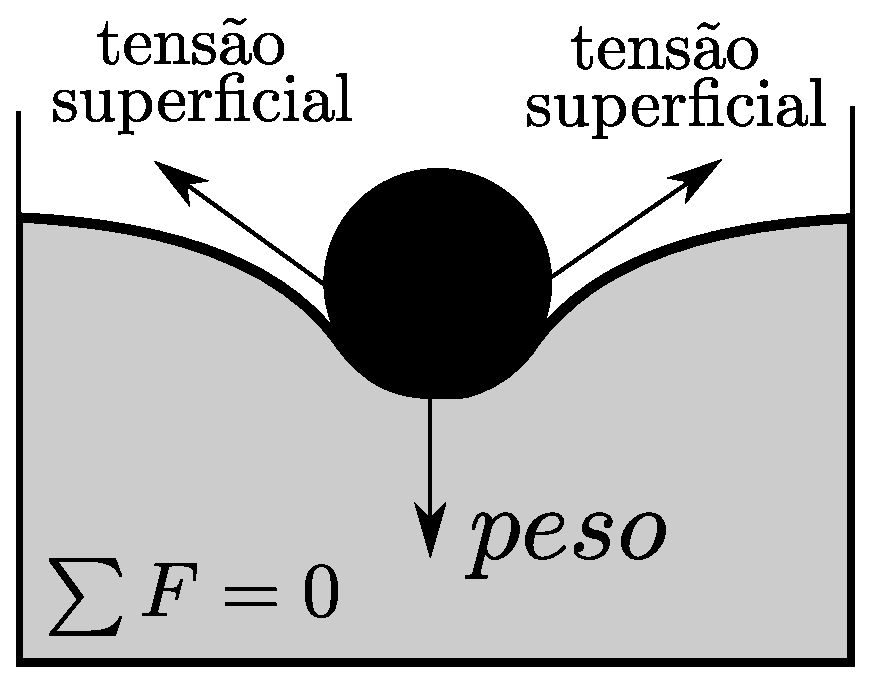
\includegraphics[angle=00, scale=0.5]{surfTension1.eps}
		\hspace{0.6cm}}
		\subfloat[capilaridade]
		{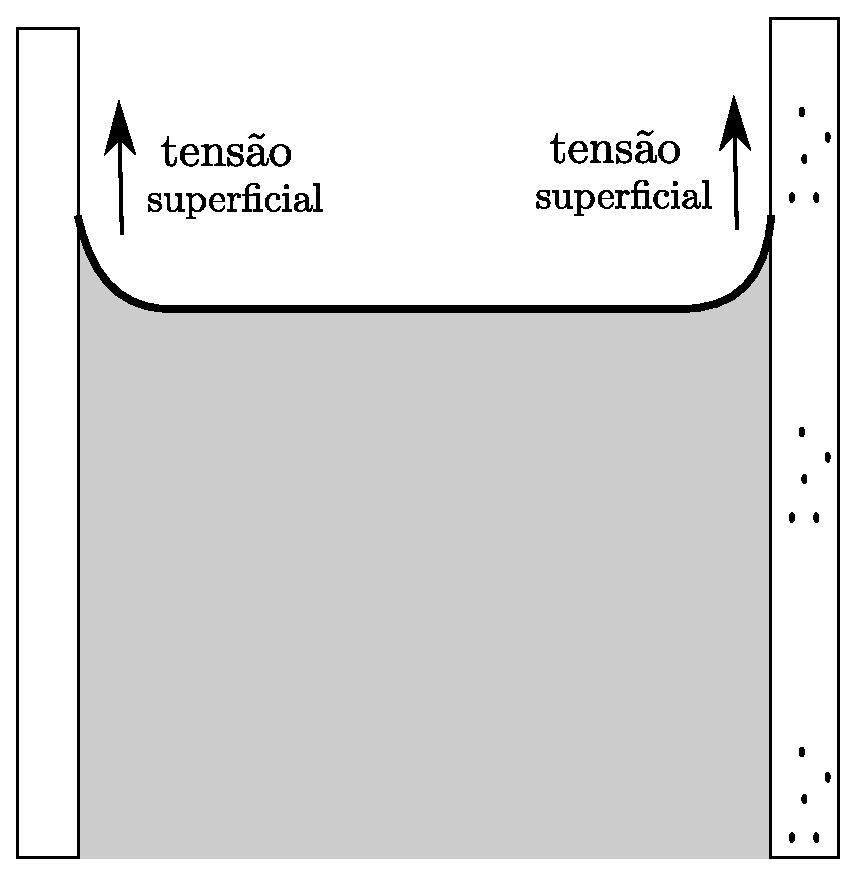
\includegraphics[angle=00, scale=0.5]{surfTension3.eps}}\\
		\subfloat[superf\'icie hidrof\'ilica]
		{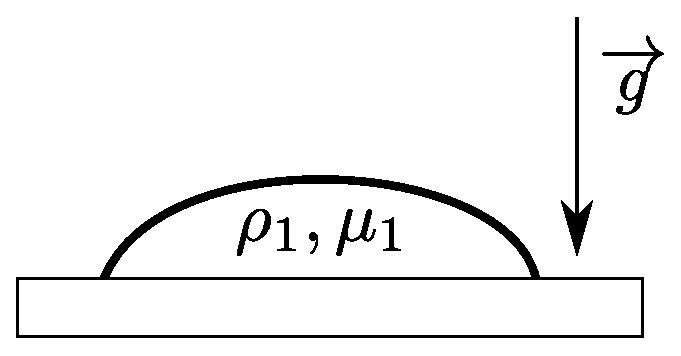
\includegraphics[angle=00, scale=0.5]{surfTension2a.eps}
		\hspace{0.6cm}}
		\subfloat[superf\'icie hidrof\'obica]
		{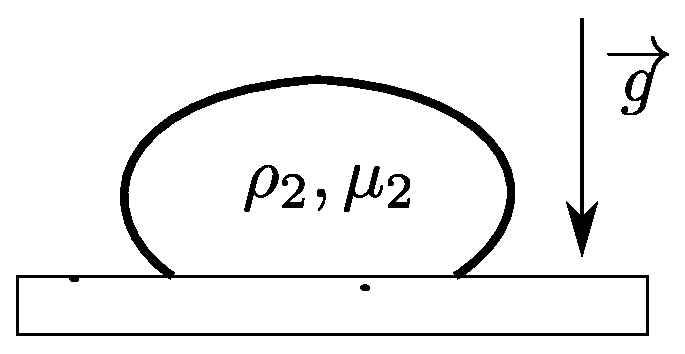
\includegraphics[angle=00, scale=0.5]{surfTension2b.eps}}
	\end{center}
	\caption{Exemplos de sistemas bif\'asicos encontrados na natureza.
	 (a) Esfera em repouso. Neste sistema a resultante das for\c cas \'e
	 zero pois o peso da esfera \'e correspondido pelo efeito da
	 tens\~ao superficial do l\'iquido. (b) Efeitos de capilaridade
	 fazem o l\'iquido subir sobre as paredes do tubo. (c) Em uma
	superf\'icie hidrof\'ilica, a gota tende a se espalhar, enquanto em
   uma (d) superf\'icie hidrof\'obica, a gota tende a ficar concentrada
  em uma \'area de contato menor.}
	\label{fig:surfTension} 
\end{figure}

%--------------------------------------------------
% \begin{wrapfigure}[10]{r}{90mm}
% %\vspace{-50pt}
%    	\begin{center}
%        	\epsfxsize=9truecm
%    		\epsffile{Hele_shaw/camadasolidificada.eps}
% 	\end{center}
% \vspace{-.6cm}
% \caption[Escoamento em uma c�lula de Hele--Shaw.]
% {Escoamento na cavidade do molde.}
% \label{fig:HS:cavidade}
% \end{wrapfigure}
%-------------------------------------------------- 

Como p\^ode ser visto, os escoamentos bif\'asicos s\~ao facilmente
encontrados na natureza. Com isso, uma boa compreens\~ao dos fen\^omenos
f\'isicos se faz necess\'aria em diversos campos da ci\^encia. Trabalhos
que datam de antes dos anos 1960 s\~ao ainda muito utilizados na
ind\'ustria, o que mostra que a ci\^encia ainda tem muito a evoluir.
Entretanto, muitos autores vem intensificando os investimentos na \'area
de escoamentos bif\'asicos, levando a um melhor entendimento e
caracteriza\c c\~ao do problema. As seguintes se\c c\~oes descrevem as
principais t\'ecnicas utilizadas por estes pesquisadores para
compreender este fascinante fen\^omeno, com \^enfase em uma revis\~ao
bibliogr\'afica de simula\c c\~oes num\'ericas e experimentais.

\section{Equa\c c\~oes de Governo}

Na literatura s\~ao encontrados dois tipos de modelos matem\'aticos para
escoamentos bif\'asicos: um fluido e dois fluidos. No modelo de dois
fluidos (\emph{two-fluids}), cada fluido \'e descrito atrav\'es de um
conjunto de equa\c c\~oes de governo. Em geral, cada fluido tem seus
pr\'oprios campos de velocidade e press\~ao e uma rela\c c\~ao
matem\'atica \'e estabelecida para o acoplamento das fases. Para o
modelo de um fluido (one-fluid), as equa\c c\~oes que modelam o
fen\^omeno f\'isico s�o as mesmas que modelam escoamentos monof\'asico,
por\'em o termo de tens\~ao superficial \'e acrescentado ao lado direto
da equa\c c\~ao de conserva\c c\~ao de quantidade de movimento (Cap. 3,
Volume 1). Este cap\'itulo focar\'a sua introdu\c c\~ao no modelo de um
fluido. Uma vez que a dedu\c c\~ao das equa\c c\~oes de conserva\c c\~ao
para escoamentos monof\'asicos se encontra no volume 1 deste livro,
tomamos a liberdade de apresentar estas equa\c c\~oes, aplicadas a
escoamentos bif\'asicos, em sua forma euleriana vetorial, para o modelo
de um fluido.

\begin{equation}
	\rho \bigg[ \ 
	\frac{\partial \rho v_x}{\partial x}+
	\frac{\partial \rho v_y}{\partial y}+
 	\frac{\partial \rho v_z}{\partial z}
	\bigg]
	=
	\rho \nabla \cdot \vvet 
	=
	0
\label{eq:cm9}
\end{equation}

Desde que $\rho \ne 0$ em todas as fases, a equa\c c\~ao de conserva\c
c\~ao de
massa \'e apresentada como:

\begin{equation}
	\nabla \cdot \vvet = 0
\label{eq:cmFinal}
\end{equation}

\noindent aqui, $\vvet$ representa o vetor de velocidades que para o caso
bidimensional contem as componentes $x$ e $y$ e no caso tridimensional
$x$, $y$ e $z$. Como mencionado anteriormente, a equa\c c\~ao de
conseva\c c\~ao
de quantidade de momento \'e modificada com a adi\c c\~ao do termo de
tens\~ao superficial $\fvet_{s}$, resultando em:

\begin{equation}
	\rho \bigg [ \frac{\partial \vvet}{\partial t} + 
	\vvet \cdot \nabla \vvet \bigg ]
	= -\nabla p + \nabla \cdot [ \mu (\nabla \vvet + \nabla \vvet^T) ] + 
	\rho \gvet +
	\fvet_{s}
\label{eq:qm16}
\end{equation} \vspace{0.0cm}

Na equa\c c\~ao acima, $\rho$ e $\mu$ representam densidade e viscosidade
respectivamente. No entanto, no modelo de um fluido (one-fluid), estes
valores permanecem constantes em cada fase, por\'em n\~ao s\~ao
necessariamente constantes em todo o espa\c co.  $t$ representa a
vari\'avel temporal, $p$ o campo de press\~ao e $\gvet$ o campo
gravitacional. 

Esta equa\c c\~ao pode ser reescrita em sua forma \emph{Lagrangiana},
tomando como base a movimenta\c c\~ao do referencial de acordo com a
movimenta\c c\~ao do fluido.

\begin{equation}
	\rho \frac{D \vvet}{D t}
	= -\nabla p + \nabla \cdot [ \mu (\nabla \vvet + \nabla \vvet^T) ] +  
	\rho \gvet +
	\fvet_{s}
\label{eq:qmFinal}
\end{equation} \vspace{0.0cm}

Neste caso, a nota\c c\~ao do lado esquerdo da equa\c c\~ao \ref{eq:qm16} \'e
compactado atrav\'es do operador derivada substantiva $D/Dt$. A
diferen\c ca dos referenciais \emph{Euleriano} e \emph{Lagrangiano} \'e
que no primeiro o referencial se encontra fixo no espa\c co, enquanto
que no segundo o referencial movimenta com a velocidade do fluido. Estes
dois referenciais ainda podem ser descritos em uma forma \'unica e
generalizada, conhecida como referencial \emph{Euleriano-Lagrangiano}
arbitr\'ario onde a referencial pode n\~ao estar nem fixo, nem
movimentando conforme o escoamento, e sim em uma velocidade
arbitr\'aria. Entretanto, a defini\c c\~ao deste referencial n\~ao est\'a
presente no escopo deste cap\'itulo. Para o leitor interessado,
recomenda-se: \cite{hughes1981} e \cite{donea1982}. 

\subsection{Adimensionaliza\c c\~ao das Equa\c c\~oes de Governo}

Esta sec\c c\~ao descreve a adimensionaliza\c c\~ao das equa\c c\~oes de
conversa\c c\~ao de massa e quantidade de movimento. Tal procedimento
melhora o entendimento e a an\'alise da influ\^encia de cada termo na
equa\c c\~ao. Duas equa\c c\~oes distintas ser\~ao apresentadas. A primeira
\'e comumente usada quando a velocidade a dimens\~ao caracter\'isticas
s\~ao conhecidas. A segunda \'e geralmente empregada para o caso de escoamentos
regidos pelo campo gravitacional, sem entrada de fluido. Neste caso a
gravidade deve ser considerada como par\^ametro conhecido, com isso a
velocidade \'e um resultado, e n\~ao uma condi\c c\~ao preestabelecida. 

As equa\c c\~oes de conserva\c c\~ao de massa e quantidade de movimento
s\~ao adimensionalizadas pela defini\c c\~ao dos seguintes par\^ametros
adimensionais:

\begin{align}
	\rho
	&=
	\rho_{\infty} \rho^* & x
	&=
	Lx^* & \qquad \gvet
	&=
	g_{\infty} \gvet^*  & \qquad \sigma
	&= \sigma_0 \sigma^*	
	\nonumber
	\\
	\mu
	&=
	\mu_{\infty} \mu^* & \vvet
	&=
	U \vvet^* & \qquad t
	&=
	\frac{L}{U}t^*  &\qquad \kappa
	&=
	\frac{1}{L}\kappa^*
	\nonumber
	\\
	p
	&=
	\rho_{\infty} U^2 p^* & \frac{\partial}{\partial t}
	&=
	\frac{U}{L}\frac{\partial}{\partial t^*} & \qquad \nabla
	&=
	\frac{1}{L}\nabla^* 
	\nonumber
\end{align}\vspace{0.0cm}

\noindent onde o sobrescrito $*$ representa as vari\'aveis
adimensionais. Seguindo o procedimento apresentado pelos Caps.~(2) e (3)
do Volume 1 deste livro, o processo de
adimensionaliza\c c\~ao das equa\c c\~oes de governo para escoamento
multif\'asico incompress\'iviel chega a:

\begin{equation}
	\nabla \cdot \vvet 
	= 
	0
\label{eq:massAdimenFinal} 
\end{equation}\vspace{0.0cm}

\begin{equation}
	\frac{\partial \vvet}{\partial t}+
	\vvet \cdot \nabla \vvet
	=
	-\nabla p + \frac{1}{Re}
	\nabla \cdot [\mu (\nabla \vvet + \nabla \vvet^{T})] +
	\frac{1}{Fr^2} \gvet +
	\frac{1}{We} \fvet_{s}
	\label{eq:momentumAdimenFinal}
\end{equation}\vspace{0.0cm}

\noindent nas equa\c c\~oes adimensionais apresentadas acima, os
n\'umeros de \emph{Reynolds} ($Re$) representa a
raz\~ao das for\c cas inercial e viscosa, o n\'umero de \emph{Froude}
($Fr$) representa a raz\~ao das for\c cas inercial e gravitacional e,
finalmente, o n\'umero de \emph{Weber} ($We$) representa a raz\~ao das
for\c cas inercial e de tens\~ao superficial.

A adimensionaliza\c c\~ao das equa\c c\~oes de governo apresentadas
consideram que a velocidade do escoamento \'e um par\^ametro conhecido.
Entretanto, em alguns casos onde a velocidade \'e consequ\^encia de uma
condi\c c\~ao e n\~ao \'e imposta diretamente no sistema, um par\^ametro de
adimensionaliza\c c\~ao diferente deve ser usado no lugar. Como exemplo pode
se citar o caso de uma bolha de g\'as em ascens\~ao em uma coluna de
l\'iquido im\'ovel. Neste sistema, o campo de velocidades \'e o
resultado, com isso n\~ao pode ser usado como referencial. Ent\~ao, a
velocidade $\vvet$ \'e comumente adimensionalizada por $\sqrt{g D}$ e o
comprimento caracter\'istico $L$ pelo di\^ametro da bolha $D$.
Substituindo estes par\^ametros na Eq.~(\ref{eq:qmFinal}), a equa\c c\~ao
final de conserva\c c\~ao de quantidade de movimento se escreve como:

\begin{equation}
	\frac{\partial \vvet}{\partial t}+
	\vvet \cdot \nabla \vvet
	=
	-\nabla p + 
	\frac{1}{N^2}
	\nabla\cdot [\mu(\nabla\vvet+\nabla \vvet^{T})] +
	\gvet +
	\frac{1}{Eo} \fvet_{s}
	\label{eq:momentumAdimenFinal2}
\end{equation}\vspace{0.0cm}

\noindent onde o n\'umero de \emph{Archimedes} ($N$) representa a
raz\~ao das for\c cas inercial e gravitacional, enquanto que o n\'umero
de \emph{E\"otv\"os} number $(Eo)$ representa a raz\~ao das for\c cas de
gravidade e tens\~ao superficial.

\section{Abordagem Num\'erica}

Em escoamentos bif\'asicos, ou \emph{two-phase flows} em ingl\^es, a
modelagem discreta da interface \'e o par\^ametro mais importante para
se obter precis\~ao nos c\'alculos. Encontra-se na literatura duas
abordagens cl\'assicas para representa\c c\~ao da interface entre dois
fluids: \emph{Euleriana} e \emph{Lagrangiana}. Estas duas abordagens
est\~ao fortemente ligadas \`a representa\c c\~ao do escoamento. Figura~(\ref{fig:interface}) representa um esquema bidimensional das
descri\c c\~oes de interface nos dois modos acima citados. 

Na descri\c c\~ao \emph{Euleriana}, tamb\'em conhecida do ingl\^es
\emph{inteface capturing}, a interface n\~ao \'e representada
explicitamente atrav\'es de objetos computacionais (n\'os, segmentos e
elementos), ao contr\'ario ela \'e definida atrav\'es de uma fun\c c\~ao de
identifica\c c\~ao de fases e deslocada atrav\'es de uma equa\c c\~ao
hiperb\'olica. Devido a sua discretiza\c c\~ao, tal equa\c c\~ao \'e uma fonte
de difus\~ao num\'erica e deve ser tratada com aten\c c\~ao. Neste tipo de
representa\c c\~ao de interface, mudan\c cas topol\'ogicas na interface,
como coalesc\^encia e ruptura, s\~ao facilmente modeladas. No entanto, a
descri\c c\~ao de todas as escalas presentes no problema f\'isico requer um
n\'umero de pontos computacionais mais elevado.

Na descri\c c\~ao \emph{Lagrangiana}, a interface que separa as duas fases
\'e representada atrav\'es de um conjunto de objetos computacionais,
tais como: n\'os, segmentos e elementos. Figura~(\ref{fig:interface}b)
ilustra um caso bidimensional onde a interface est\'a representada por
tais objetos como parte do dom\'inio num\'erico. Como pode ser visto, a
interface n\~ao divide nenhum elemento, com isso nenhum tratamento
especial \'e necess\'ario para modelar fortes diferen\c cas de
propriedades f\'iscias como viscosidade e densidade. Adicionalmente \`a
esta abordagem, a interface \'e representada sem qualquer difus\~ao, ou
seja, esta \'e definida com espessura zero, assemelhando-se \`a uma fiel
representa\c c\~ao da realidade. O movimento da interface \'e feito
atrav\'es do pr\'oprio campo de velocidade, sem o aux\'ilio de qualquer
equa\c c\~ao adicional. 


\begin{figure}[ht!]
		\subfloat[]{\label{fig:interface1}
		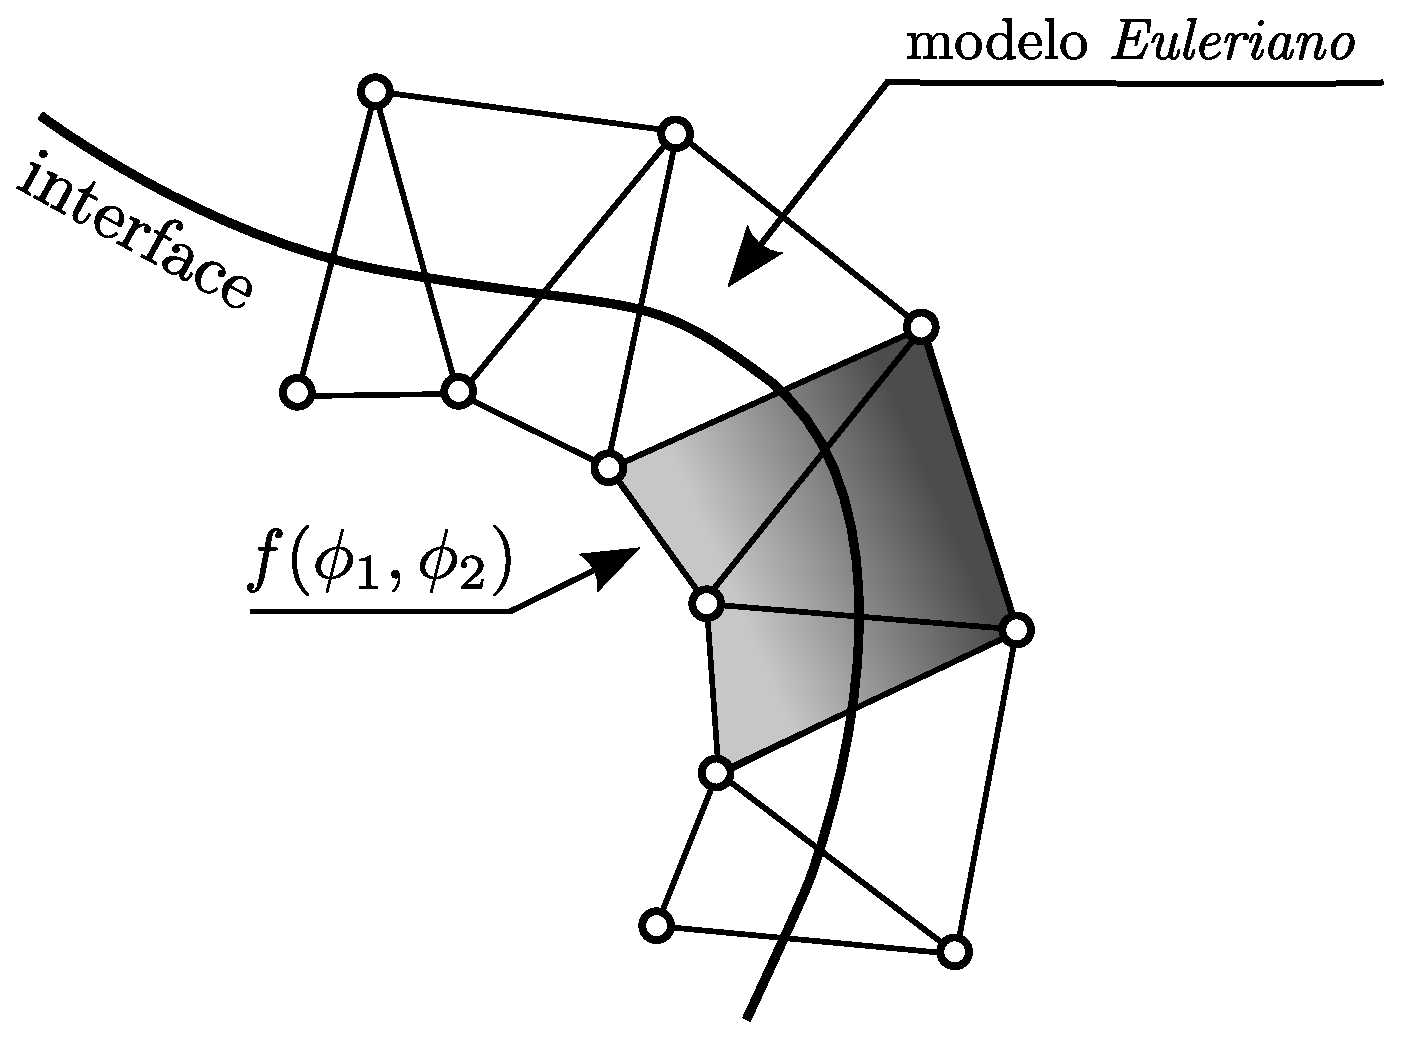
\includegraphics[scale=0.32]{interface1.eps}}
		\subfloat[]{\label{fig:interface2}
		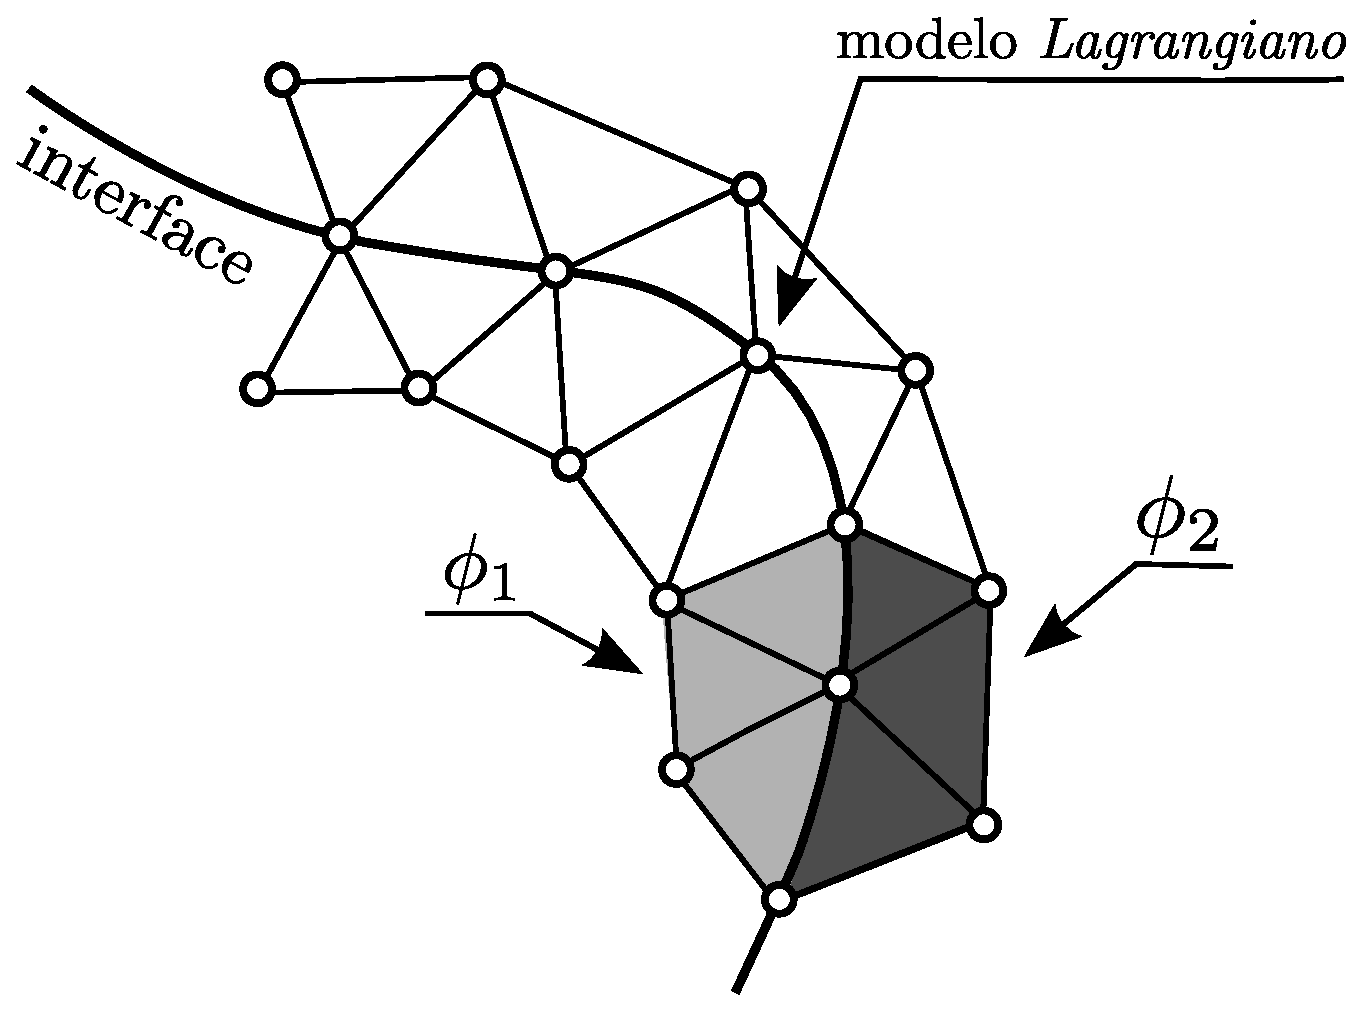
\includegraphics[scale=0.32]{interface2.eps}}
	\caption[Representa\c c\~ao da interface em escoamentos
	 bif\'asicos.]{Representa\c c\~ao da interface em escoamentos
	 bif\'asicos. (a) Na descri\c c\~ao \emph{Euleriana}, a interface
	 entre os fluidos \'e definida em uma posi\c c\~ao arbitr\'aria em
	 rela\c c\~ao aos elementos. Diferentemente, (b) o descri\c c\~ao
	 \emph{Lagrangiana} representa a interface atrav\'es de pontos
	 pertencentes \`a malha computacional atrav\'es da defini\c c\~ao de
	 objectos, tais quais n\'os, segmentos e elementos, obtendo assim
	 uma representa\c c\~ao precisa da interface.}
	\label{fig:interface} 
\end{figure}

Entre as descri\c c\~oes \emph{Euleriana} e \emph{Lagrangiana},
diferentes t\'ecnicas est\~ao dispon\'iveis para a modelagem de
escoamentos bif\'asicos. Cada metodologia particular garante um conjunto
de caracter\'isticas com diferentes n\'iveis de programa\c c\~ao. Abaixo
ser\~ao apresentados os m\'etodos mais comumente encontrados na
literatura de escoamentos bif\'asicos.

% --------------------------------------------------------------- %
%                     Volume of Fluid - VOF                       %
% --------------------------------------------------------------- %
Em 1980, o m\'etodo volume de fluido (\emph{Volume of Fluid} ou VOF na
sigla em ingl\^es) foi proposto por \cite{hirt1981}, no qual consiste na
descri\c c\~ao de cada fase atrav\'es do volume de fluido ocupado em cada
elemento computacional. Os inteiros ``0'' e ``1'' s\~ao atribu\'idos
para definir a regi\~ao ocupada na totalidade por cada fluido e valores
intermedi\'arios s\~ao atribu\'idos nos elementos onde a interface \'e
definida. Devido \`a descontinuidade proveniente desta metodologia, uma
alta precis\~ao n\~ao pode ser garantida no c\'alculo da curvatura e dos
vetores normais \`a interface. Figura~(\ref{fig:vof-interface}) mostra
um esquema bidimensional do m\'etodo \emph{VOF} em uma malha retangular
estruturada.

\begin{figure}[ht!]
		\subfloat[]{\label{fig:vof1}
		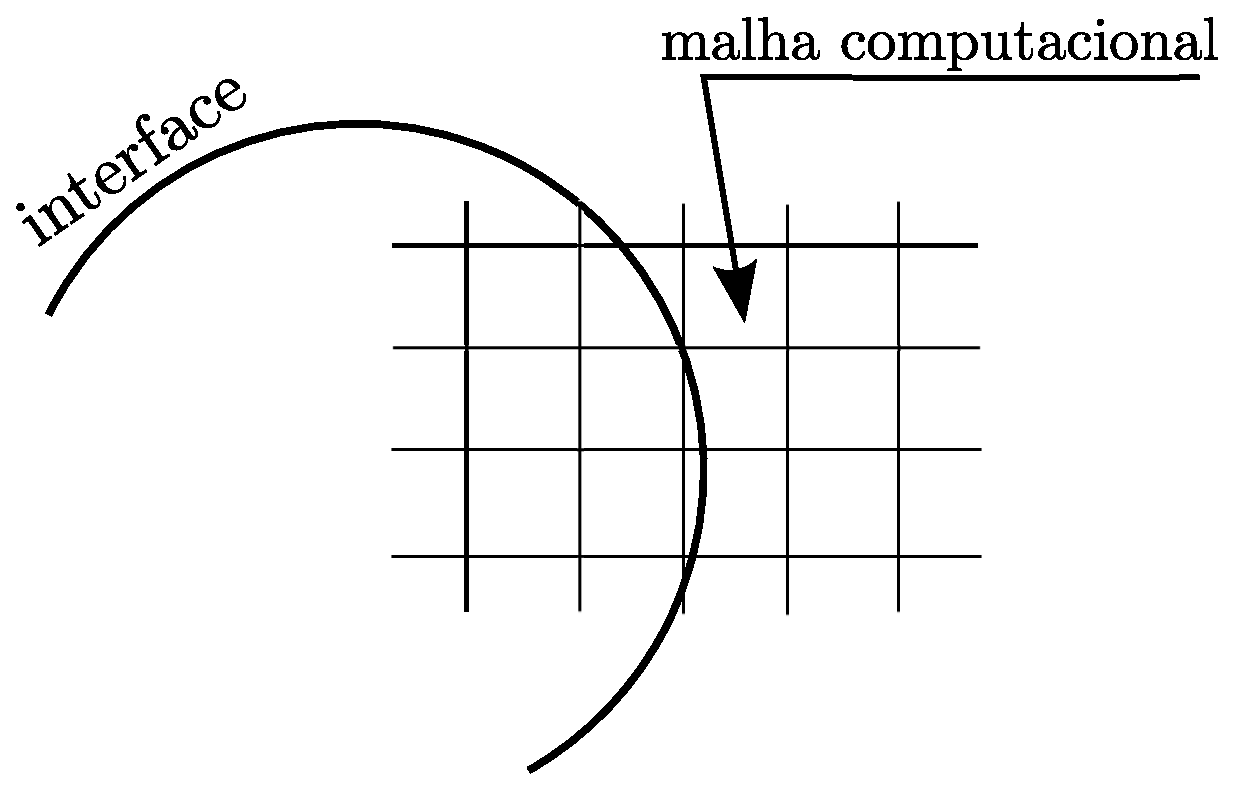
\includegraphics[scale=0.45]{vof.eps}}
		\subfloat[]{\label{fig:vof2}
		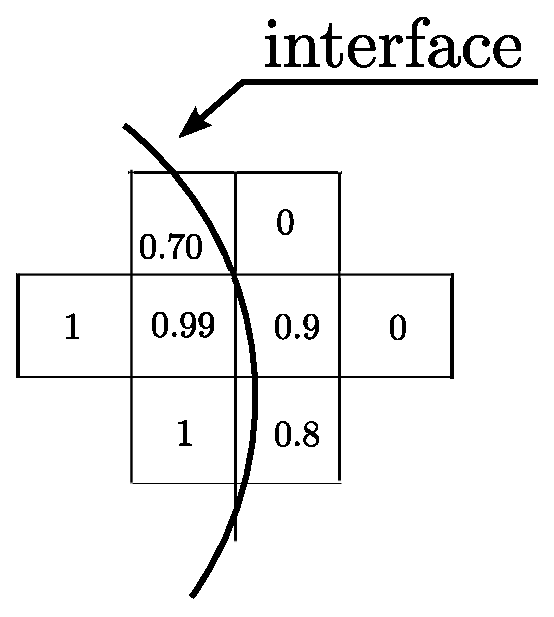
\includegraphics[scale=0.6]{vofzoom.eps}}
		\caption[Representa\c c\~ao da interface no m\'etodo
		 \emph{VOF}.]{Representa\c c\~ao da interface no m\'etodo
		 \emph{VOF}. (a) A interface entre os fluidos \'e definida
		 implicitamente e localizada em algum lugar entre elementos
		 computacionais. (b) A fun\c c\~ao \emph{VOF} \'e constru\'ida
		 considerando-se o volume ocupado por cada fluido em cada
	     elemento computacional.}
	\label{fig:vof-interface} 
\end{figure}

Um modelo bidimensional foi desenvolvido por \cite{tomiyama1993} e
depois extendido a escoamentos tridimensionais \cite{tomiyama1997}. O
c\'odigo tridimensional incluiu uma nova metodologia baseada no m\'etodo
de rastreamento de part\'iculas (\emph{particle tracking method} em
ingl\^es), na qual os efeitos de cada fase s\~ao considerados na outra
fase e vice-versa. Testes foram realizados para investiga\c c\~ao de bolha
em ascen\c c\~ao em um fluido parado. Uma grande faixa de n\'umeros
adimensionais \emph{E\"otv\"os} e \emph{Morton} foram testadas e
comparadas a resultados experimentais, com isso provando a capacidade do
c\'odigo em capturar os efeitos observados em fluidos com diferentes
propriedades. 

Em \cite{chen1998}, um modelo de escoamento bif\'asico baseado no
m\'etodo \emph{VOF} foi desenvolvido para simular escoamentos com
grande diferen\c ca na rela\c c\~ao de densidades. O modelo de for\c ca de
superf\'icie cont\'inua (continuum surface force model - CSF  em
ingl\^es) foi usado para obter-se os efeitos da tens\~ao superficial nas
equa\c c\~oes de Navier-Stokes. A coalesc\^encia de bolhas e a bolha em
ascen\c c\~ao foram investigadas para valida\c c\~ao do c\'odigo num\'erico com
dados de literatura dispon\'ivies. O m\'etodo proposto apresentou boa
concord\^ancia com dados experimentais. 

Um modelo de escoamento bif\'asico bidimensional foi apresentado em 
\cite{ginzburg2000} com utiliza\c c\~ao do m\'etodo \emph{VOF} e um m\'etodo
de elementos finitos escalonado. Esta metodologia foi baseada em uma
classe de elementos facilmente encontrada no m\'etodo de elementos
finitos, chamada \emph{Crouzeix-Raviart}. Adicionalmente, um refinamento
de malha adaptativo foi utilizado para obter-se uniformidade nos
elementos de malha pr\'oximo \`a interface. Foram executados testes
est\'aticos e din\^amicos, como a bolha em ascens\~ao, encontrando-se
boas compara\c c\~oes a resultados experimentais.

Em \cite{wu1998} foi desenvolvido um modelo bidimensional e
axisim\'etrico utilizando os m\'etodo de elementos finitos para
simula\c c\~ao de escoamentos bif\'asicos atrav\'es do m\'etodo \emph{VOF}.
Um modelo modificado da for\c ca de superf\'icie cont\'inua (\emph{CSF})
foi proposto para tratar o termo de tens\~ao superficial nas equa\c
c\~oes de Navier-Stokes. Tal modelo contorna as dificuldades na
aproxima\c c\~ao da curvatura da interface e, com isso, facilita seu
c\'alculo. Resultados foram comparados com sucesso a diferentes casos
como rompimento de barragem (\emph{Dam breaking}), gota oscilante e
bolhas estacion\'arias.

% --------------------------------------------------------------- %
%                         Level-Set - LS                          %
% --------------------------------------------------------------- %
O m\'etodo de Level-Set (LS) na din\^amica de fluidos foi primeiramente
apresentado por \cite{osher1988} e se tornou uma importante ferramenta
para modelagem de escoamentos bif\'asicos. Neste m\'etodo a interface
\'e representada por uma fun\c c\~ao dist\^ancia de n\'ivel zero que \'e
movimentada pelo campo de velocidades. A curvatura e os vetores normais
\`a interface s\~ao convenientemente calculados com a ajuda da mesma
fun\c c\~ao dist\^ancia, com isso uma modelagem direta da tens\~ao
superficial \'e realizada com sucesso. Apesar de sua recente apari\c
c\~ao nos modelos de escoamento bif\'asico, o m\'etodo de Level-Set
provou-se ser um dos mais importantes modelos de din\^amicas
interfaciais. Figura~(\ref{fig:ls}) mostra a representa\c c\~ao das
fun\c c\~oes dist\^ancia e Level-Set em um caso bidimensional com
dom\'inio em forma de quadrado. A fun\c c\~ao dist\^ancia \'e calculada
atrav\'es da norma 2 do espa\c co Euclidiano em cada n\'o da malha e sua
respectiva menor dist\^ancia \`a interface separando os fluidos,
matematicamente $\xvet-\xvet_I$, onde $\xvet$ \'e o n\'o da malha e
$\xvet_I$, o n\'o mais pr\'oximo da interface. A mesma fun\c c\~ao
dist\^ancia \'e usada para o c\'alculo da fun\c c\~ao de Level-Set, que
n\~ao \'e nada mais que uma vers\~ao com sinais positivo e negativo,
representando o que est\'a em uma fase e em outra. As duas fun\c c\~oes
representam a interface quando o valor coincide com zero. 

\begin{figure}[ht!]
		\subfloat[]{\label{fig:distance}
		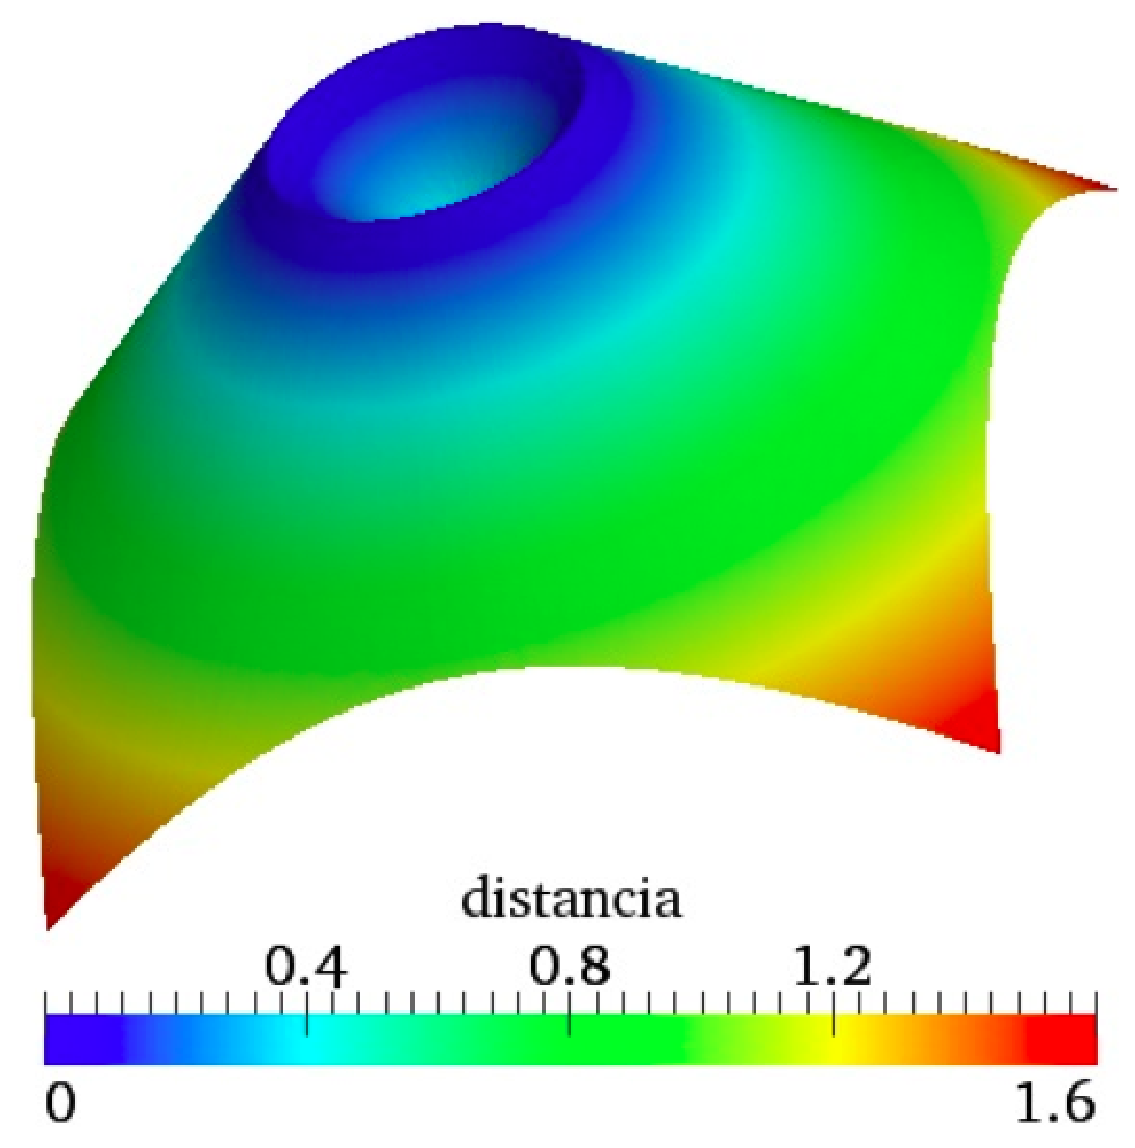
\includegraphics[scale=0.33]{distance.eps}}
		\hspace{0.5cm}
		\subfloat[]{\label{fig:level-set}
		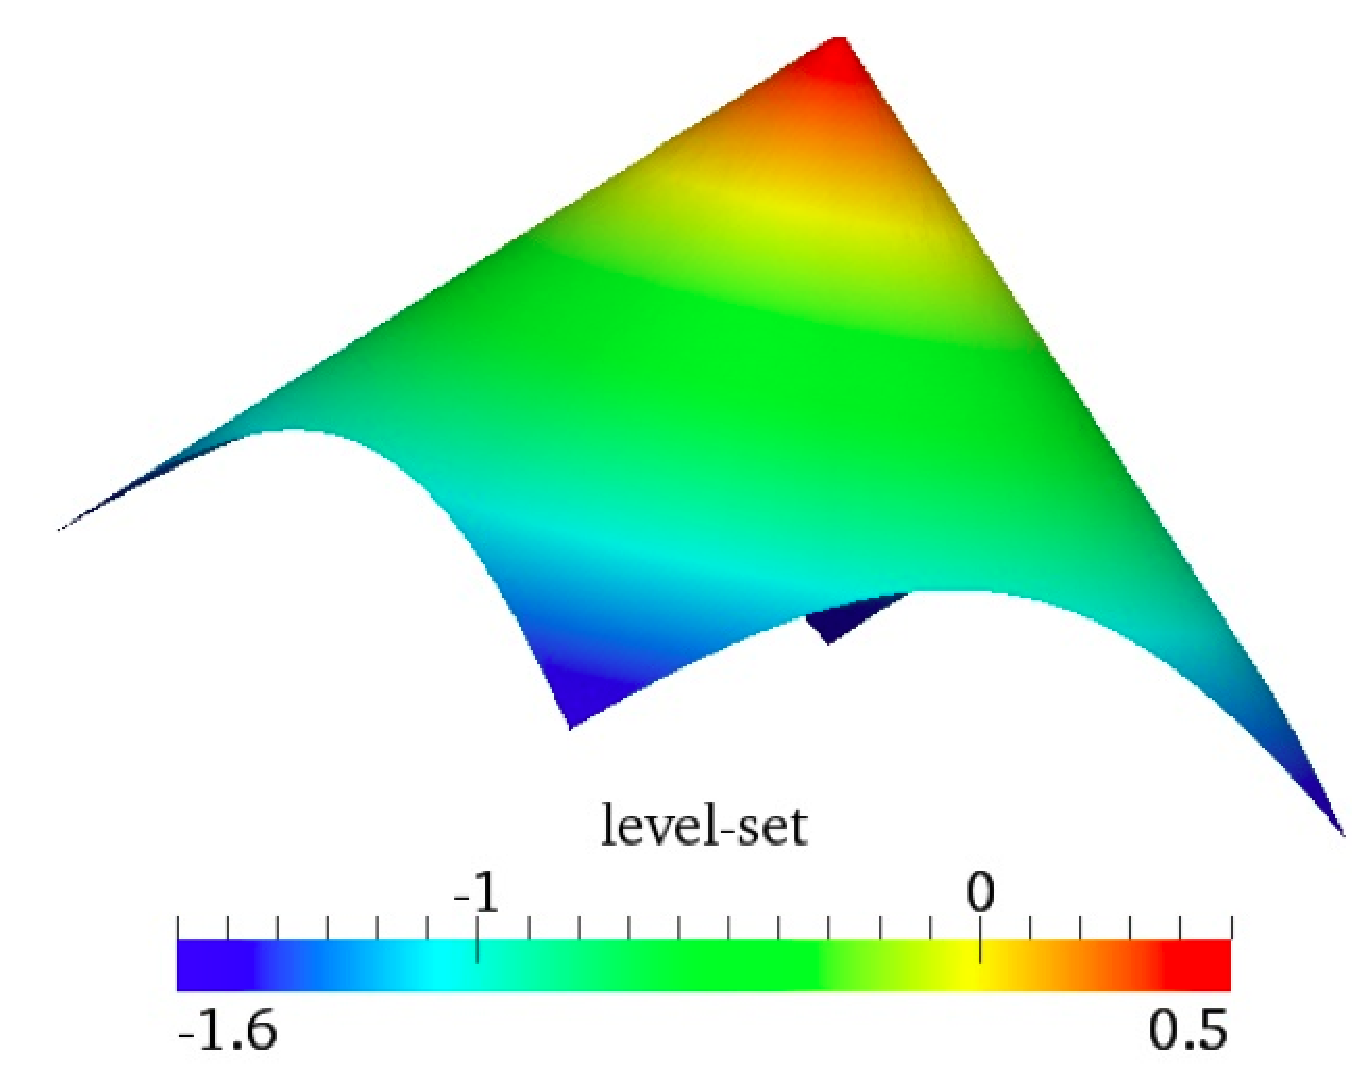
\includegraphics[scale=0.33]{level-set.eps}}
	\caption[Representa\c c\~ao das fun\c c\~oes dist\^ancia e
	 Level-Set.]{Representa\c c\~ao das fun\c c\~oes dist\^ancia e
	 Level-Set. A interface entre os fluidos \'e localizada no meio do
	 dom\'inio computacional. (a) A fun\c c\~ao dist\^ancia \'e criada
	 atrav\'es do c\'alculo da dist\^ancia de cada n\'o da malha $\xvet$
	 para seu correspondente n\'o da interface mais pr\'oximo $\xvet_I$.
	 (b) A fun\c c\~ao de Level-Set \'e representada como sendo a fun\c
	 c\~ao dist\^ancia com sinais positivo e negativo correspondentes
	 \`a localiza\c c\~ao do fluido.}
	\label{fig:ls} 
\end{figure}

O m\'etodo de Level-Set em escoamentos bif\'asicos foi primeiramente
desenvolvido por  \cite{sussman1994} e seguido por muitos outros
autores. Eles propuseram um esquema de segunda ordem baseado em um
esquema \emph{upwind}/proje\c c\~ao para o c\'alculo da solu\c c\~ao das
equa\c c\~oes de Navier-Stokes para fluidos imisc\'iveis. Foi mostrado
que a conserva\c c\~ao de mass \'e apenas garantida se a fun\c c\~ao de
Level-Set \'e reinicializada preferencialmente em todo passo de tempo.
Eles realizaram significativos testes com bolhas e gotas para valida\c
c\~ao desta nova metodologia. Adicionalmente, \cite{sussman1997}
apresentaram sua vers\~ao extendida para o caso tridimensional de
superf\'icie livre. Novamente, testes foram realizados com sucesso para
valida\c c\~ao desta nova extens\~ao atrav\'es de importantes casos,
tais quais gota est\'atica e gota oscilante em gravidade zero.

O acoplamento dos m\'etodos de Level-Set e de elementos finitos foi
apresentado por \cite{quecedo2001}, no qual as equa\c c\~oes de
escoamento de fluido foram discretizadas em uma malha triangular. Foi
proposto um m\'etodo de passo de tempo fracion\'ario no qual foi usado
para estabilizar press\~ao  e velocidade, por consequ\^encia permitindo
o uso do mesmo elemento finito para discretiza\c c\~ao  de ambas as
grandezas f\'isicas. Grandes diferen\c cas em densidade foram testadas
com sucesso e comparados a outros testes cl\'assicos na literatura.

Uma formula\c c\~ao de elementos finitos estabilizada e acoplada ao
m\'etodo de Level-Set foi desenvolvida para o c\'alculo da din\^amica de
bolhas em \cite{nagrath2005}. Um m\'etodo tipo Petrov-Galerkin foi
tamb\'em utilizado para discretizar as equa\c c\~oes de conserva\c c\~ao
de quantidade de movimento. Coalesc\^encia e ascens\~ao  de bolhas
foram estudadas e comparadas com a metodologia proposta.

Um m\'etodo num\'erico foi proposto em \cite{marchandise2006} para a
simula\c c\~ao tridimensional incompress\'ivel de escoamentos bif\'asicos. O
m\'etodo de Level-Set foi utilizado com sucesso junto ao m\'etodo de
elementos finitos estabilizado para a solu\c c\~ao das equa\c c\~oes de
Navier-Stokes. Os resultados foram ent\~ao comparados com muitos
exemplos num\'ericos comumentes encontrados na literatura, tais quais
escoamento de \emph{Poiseuille}, instabilidade de Rayleigh-Taylor,
ruptura de barragem etc. Todos os testes apresentaram boa concord\^ancia
com a literatura.

Apesar da grande utiliza\c c\~ao  do m\'etodo de Level-Set, resultados
mostraram que a implementa\c c\~ao direta deste m\'etodo ocasiona excessiva
difus\~ao num\'erica, com isso a reinicializa\c c\~ao da fun\c c\~ao de
Level-Set se faz obrigat\'oria em todo o passo tempo. Uma outra
alternativa, adotada por muitos autores, \'e o acoplamento do m\'etodo
de Level-Set com o m\'etodo VOF, formando CLSVOF (\emph{coupled
Level-Set Volume-of-Fluid} em ingl\^es). Esta nova metodologia (ver
\cite{bourlioux1995}, \cite{sussman2000} and \cite{nichita2010a}) utiliza
as principais caracter\'isticas de cada m\'etodo separado, com isso a
curvatura e os vetores normais s\~ao  calculados atrav\'es da fun\c c\~ao de
Level-Set enquanto que a interface \'e capturada a partir da fun\c c\~ao
VOF. Consequentemente, os erros de conserva\c c\~ao de massa presentes no
m\'etodo de Level-Set e o pobre c\'alculo de curvatura proveniente do
m\'etodo VOF s\~ao eliminados.

% --------------------------------------------------------------- %
% Front-tracking                                                  %
% --------------------------------------------------------------- %

Ao contr\'ario dos m\'etodos Level-Set e VOF, a descri\c c\~ao
\emph{Lagrangiana} define a interface entre fluidos explicitamente
atrav\'es de elementos computacionais. Tal descri\c c\~ao \'e conhecida como
rastreamento de interface (\emph{interface tracking} no ingl\^es).
Dentro desta classe de m\'etodos, \emph{volume-tracking} e
\emph{front-tracking} s\~ao os que mais se destacam na literatura. O
primeiro utiliza part\'iculas marcadoras para reconstru\c c\~ao da interface,
combinando precis\~ao e rigor com relativamente baixo custo de
investimento (\cite{harlow1965},\cite{amsden1970}). O segundo,
primeiramente implementado por \cite{glimm1988}, representa a interface
atrav\'es de um conjunto de n\'os interconectados que se movem de acordo
com o escoamento calculado no referencial \emph{Euleriano}. Tal
descri\c c\~ao fornece uma representa\c c\~ao definida da interface com alta
precis\~ao, entretanto sua desvantagem est\'a na necessidade de um
tratamento explicito quando a interface apresenta mudan\c cas
topol\'ogicas, como no caso de coalesc\^encia e ruptura de interface.

Em \cite{unverdi1992}, uma nova metodologia para simula\c c\~ao de
escoamentos multif\'asicos foi descrita. As equa\c c\~oes foram
discretizadas atrav\'es do m\'etodo de diferen\c cas finitas em uma
malha estacion\'aria, com a interface definida explicitamente por um
conjunto de objetos geom\'etricos tais como tri\^angulos, segmentos e
pontos. Apesar da malha computacional de fundo ser est\'atica
(descri\c c\~ao \emph{Euleriana}), a malha de interface se movia com a
velocidade proveniente do escoamento. Os vetores normais \`a interface
foram calculados a partir de fun\c c\~oes trigonom\'etricas em cada
elemento da superf\'icie e a curvatura foi calculada atrav\'es de uma
aproxima\c c\~ao da indicatrix \emph{Dupin} na superf\'icie. Por apresentar
uma descri\c c\~ao explicita da interface, tal metodologia definiu com
precis\~ao a superf\'icie que separa os fluidos, entretanto as
propriedades dos fluidos n\~ao foram precisamente definidas,
necessitando ent\~ao de um tratamento num\'erico especial.  

Um modelo Level-Set \emph{Lagrangiano} foi proposto por \cite{souza2004}
para simula\c c\~ao de escoamentos incompress\'iveis bif\'asicos. As
esqua\c c\~oes de governo foram discretizadas atrav\'es do m\'etodo de
\emph{Galerkin} e elementos finitos, enquanto que o sistema linear
resultante for tratado atrav\'es do m\'etodo da proje\c c\~ao, visando
desacoplar velocidade e press\~ao. A interface entre fluidos era
representada pela pr\'opria malha do dom\'inio e ent\~ao movida pelo
campo de velocidade. Tal modelo dispensa o uso de uma equa\c c\~ao
hiperb\'olica adicional, uma vez que a interface \'e descrita por pontos
e segmentos da pr\'opia malha computacional bidimensional. O controle de
malha foi feito atrav\'es de procedimentos padr\~oes tais quais
\emph{flipping}, adi\c c\~ao e remo\c c\~ao de arestas e n\'os. Pela
defini\c c\~ao da fun\c c\~ao de Level-Set $\phi$, foi poss\'ivel
calcular diretamente a curvatura e os vetores normais \`a interface
atrav\'es das express\~oes: $\kappa=\nabla \cdot(\nabla \phi/|\nabla
\phi|)$ e $\nvet = \nabla \phi / |\nabla \phi|$, consecutivamente. Com
isso, para satisfazer o balan\c co de for\c ca discreto entre press\~ao
e tens\~ao superficial, o gradiente da fun\c c\~ao de \emph{Heaviside}
$\nabla H$ foi usado como substituto da fun\c c\~ao Delta de Dirac
$\delta$, encontrado no modelo de for\c ca de superf\'icie continuo
(CSF). Tal abordagem \'e comumente encontrada em modelos
\emph{Eulerianos}, por\'em mostrou-se adequado para m\'etodos do tipo
\emph{Interface-tracking}, uma vez que o salto de press\~ao atrav\'es da
interface foi precisamente calculado.

O grupo da Universidade de Massachustts sugeriu um modelo completo de
malha din\^amica para simula\c c\~ao de escoamentos tipo superf\'icie livre
e bif\'asicos (\cite{perot2003},\cite{quan2006}), no qual difere da
abordagem de malha fixa. Neste caso, a discretiza\c c\~ao das equa\c c\~oes
de governo foi feita sobre uma malha n\~ao estruturada com o aux\'ilio
de um m\'etodo de passo fracion\'ario exato. Tal t\'ecnica melhora a
defini\c c\~ao da interface, uma vez que o salto de propriedades f\'isicas
\'e mantido definido. A valida\c c\~ao da metodologia foi realizada com
sucesso atrav\'es de v\'arios testes num\'ericos comparativos, mostrando
que a t\'ecnica pode ser utilizada para modelagem de escoamentos
bif\'asicos com precis\~ao.

Um novo m\'etodo de malha que se move junto ao campo de velocidades \'e
proposto por \cite{anjos2012}. Neste, as equa\c c\~oes de governo s\~ao
discretizadas atrav\'es do m\'etodo de elementos finitos, usando a
descri\c c\~ao generalizada arbitr\'aria \emph{Euleriana-Lagrangiana}. Este
m\'etodo tamb\'em permite uma representa\c c\~ao precisa da interface, uma
vez que esta \'e definida atrav\'es de elementos computacionais e
pertencentes a malha do dom\'inio. V\'arios testes e valida\c c\~oes
foram apresentados, mostrando que a metodologia descreve com precis\~ao
escoamentos bif\'asicos.

\section{Abordagem Emp\'irica ou Experimental}

Para iniciarmos a introdu\c c\~ao \`as t\'ecnias experimentais, passamos
pela defini\c c\~ao de importantes par\^ametros utilizados na
caracteriza\c c\~ao do escoamentos bif\'aiscos. A seguir, ser\~ao
identificados padr\~oes encontrados frequentemente em escoamentos
multif\'asicos em canais verticais e horizontais. \'E importante notar
que a literatura dispon\'ivel em escoamentos com mais de uma fase \'e
extenso e n\~ao se limita aos exemplos introdut\'orios apresentados
neste cap\'itulo. Ao leitor que deseja aprofundar tais conceitos,
sugerimos \cite{collier1996}, \cite{whalley1987} e \cite{carey2007}.

\subsection{T\'itulo de vapor}

O t\'itulo de vapor ($x$) \'e definida como sendo a raz\~ao da vaz\~ao
m\'assica de vapor ($\dot{M}_G$) dividida pela vaz\~ao m\'assica total
($\dot{M}_G+\dot{M}_L$):

\begin{equation}
	x = \frac{\dot{M}_G}{\dot{M}_G+\dot{M}_L}
\end{equation}

Quando o escoamento \'e adiab\'atico, ou seja n\~ao h\'a transfer\^encia
de calor, se torna necess\'ario a medida de vaz\~ao m\'assica para cada
fase, com isso o t\'itulo de vapor \'e determinada para todo o tubo. Se
o tubo \'e aquecido e fluxos de massa s\~ao notados no sistema, o
t\'itulo de vapor aumentar\'a na dire\c c\~ao do escoamento. No
entanto, para o caso de resfriamento do tubo e, consequentemente, a
condensa\c c\~ao do vapor, o t\'itulo de vapor diminuir\'a na dire\c
c\~ao do escoamento.

\subsection{Velocidades}

Em escoamentos multif\'asicos existem um grande n\'umero de velocidades
que podem ser definidas experimentalmente. Ainda, como os fluidos
est\~ao em fases distintas, diferentes velocidades podem ser
encontradas, sugerindo tamb\'em o uso de velocidade relativa como base
para caracteriza\c c\~ao da velocidade do escoamento. A seguir s\~ao
definidas algumas importantes velocidades encontradas na literatura.

\begin{itemize}
	\item Velocidade Verdadeira m\'edia (\emph{True average velocity}):
	\'e a velocidade em que cada fase se movimenta no escoamento.
	\item Velocidade superficial (\emph{Superficial velocity}:
	tamb\'em conhecida como fluxo volum\'etrico, \'e definida como a
	raz\~ao do fluxo de velocidade da fase considerada pela \'area
	transversal total do escoamento multif\'asico.
	\item Velocidade de deriva (\emph{Drift velocity}): raz\~ao da
	velocidade verdadeira m\'edia pela velocidade superficial total.
\end{itemize}

\subsection{Fluxo de massa}

O fluxo de massa ($G$) \'e definido como sendo a vaz\~ao m\'assica total
($\dot{M}$) divida pela \'area transversal do escoamento:

\begin{equation}
	G = \frac{\dot{M}}{A}
\end{equation}

\noindent onde a express\~ao acima representa a rela\c c\~ao entre a
velocidade m\'edia do escoamento multiplicada pela densidade m\'edia. A
unidade usual de fluxo de massa \'e $[kg/m^2 s]$.

\subsection{Fra\c c\~ao de vazios}

A fra\c c\~ao de vazios $\epsilon$, ou \emph{Void Fraction} em ingl\^es, \'e
um dos par\^ametros mais importantes para caracteriza\c c\~ao de escoamentos
multif\'asicos. Este tamb\'em \'e de grande import\^ancia para a
determina\c c\~ao de outros par\^ametros, tais como viscosidade e densidade
em escoamentos multif\'asicos, obten\c c\~ao de velocidade m\'edia relativa
e, tamb\'em, como ferramenta fundamental em modelos de previs\~ao de
transi\c c\~ao de padr\~oes de escoamentos. 

Na literatura existem v\'arias defini\c c\~oes para especifica\c c\~ao de
fra\c c\~ao de volume (veja \cite{thome2008}). Aqui ser\~ao apresentadas as
principais defini\c c\~oes de fra\c c\~ao de vazios: local, cordal,
transversal e volum\'etrica. 

\begin{equation}
	\epsilon_{local}(r,t) 
	= 
	\frac{1}{t} \int_t P_k(r,t) dt
\end{equation}

A fra\c c\~ao de vazios local $\epsilon_{local}$ \'e tipicamente medida
atrav\'es de um feixe radioativo brilhante que atravessa o tubo onde o
escoamento multif\'asico est\'a localizado. Atrav\'es da absor\c c\~ao de
luz neste feixe no outro lado do tubo, \'e poss\'ivel medir o
comprimento da fase gasosa. A vaz\~ao de vazios local \'e ent\~ao
determinada por: 

\begin{equation}
	\epsilon_{chordal} = \frac{L_G}{L_G+L_L}
\end{equation}

\noindent onde $L_G$ \'e o comprimento de linha na fase gasosa e $L_L$
na fase l\'iquida.

A fra\c c\~ao de vazios transversal $\epsilon_{trans}$, ou
\emph{cross-sectional} em ingl\^es, \'e medida a partir de meios
\'oticos ou atrav\'es de medidas indiretas, tal como a capacit\^ancia
el\'etrica de uma fase l\'iquida condutora. Esta fra\c c\~ao \'e definida
como:

\begin{equation}
	\epsilon_{trans} = \frac{A_G}{A_G+A_L}
\end{equation}

\noindent onde $A_G$ \'e a \'area ocupada da fase gasosa e $L_L$
da fase l\'iquida.

A fra\c c\~ao de vazios volum\'etrica $\epsilon_{vol}$ \'e medida geralmente
atrav\'es de mecanismos de armadilha para os fluidos, onde por um
instante breve a amostra fica armazenada, possibilitando a medida da
quantidade de g\'as e l\'iquido diretamente. Esta fra\c c\~ao \'e ent\~ao
definida como:

\begin{equation}
	\epsilon_{vol} = \frac{V_G}{V_G+V_L}
\end{equation}

\noindent onde $V_G$ \'e o volume ocupado da fase gasosa e $L_L$
da fase l\'iquida.

\subsection{Escoamentos verticais}

Os pad\~oes de escoamentos para cima em tubos verticais \'e apresentado
esquematicamente na Fig.~(\ref{fig:vertical}). As diferen\c cas
b\'asicas observadas experimentalmente s\~ao descritas a seguir. \'E
importante notar que a utiliza\c c\~ao de cada padr\~ao de escoamento
depende da sua aplica\c c\~ao. 

\begin{figure}[h!]
	\begin{center}
		\subfloat[Bolhas]
		{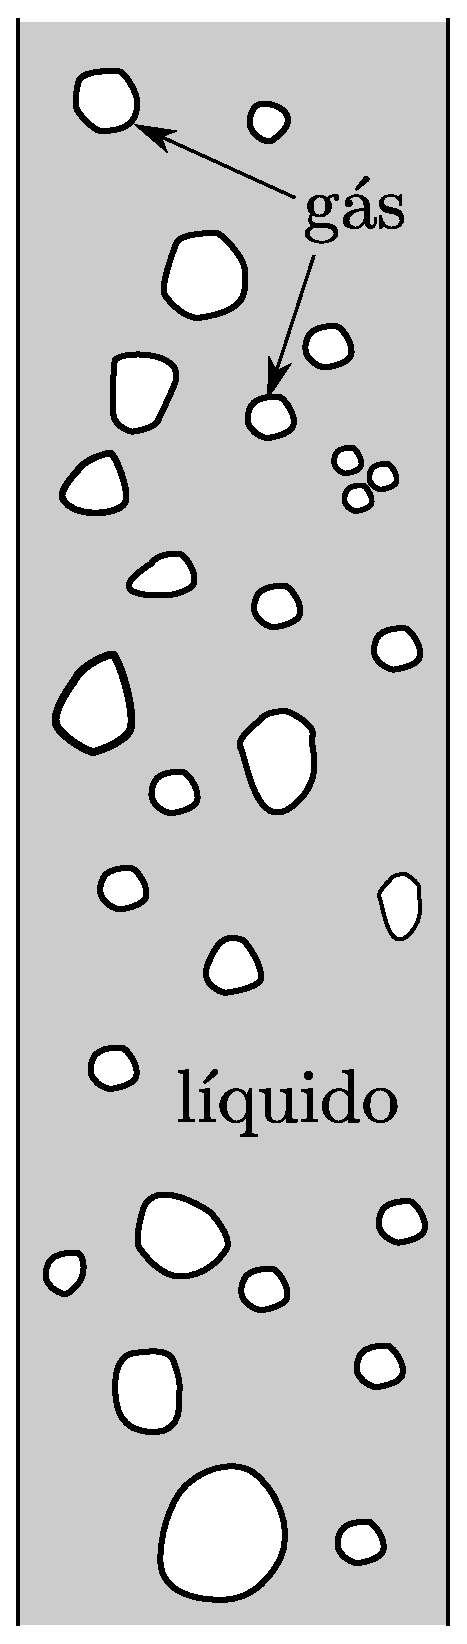
\includegraphics[angle=00, scale=0.3]{v_bubbly.eps}
		\hspace{0.8cm}}
		\subfloat[Golfada]
		{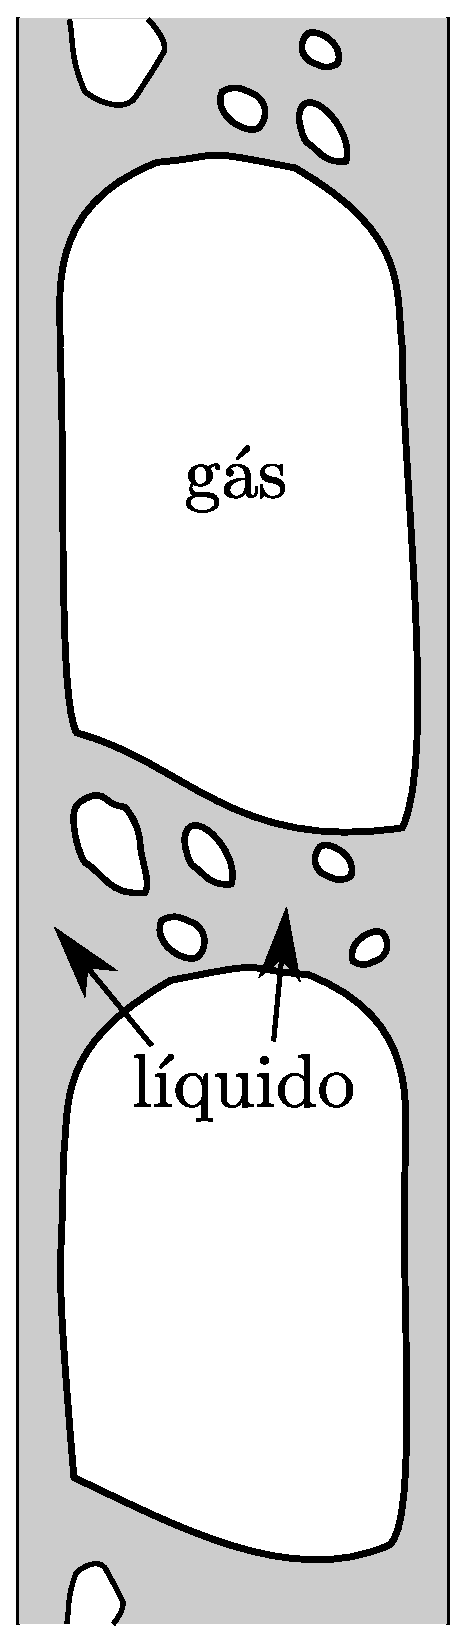
\includegraphics[angle=00, scale=0.3]{v_slug.eps}
		\hspace{0.8cm}}
		\subfloat[Batido]
		{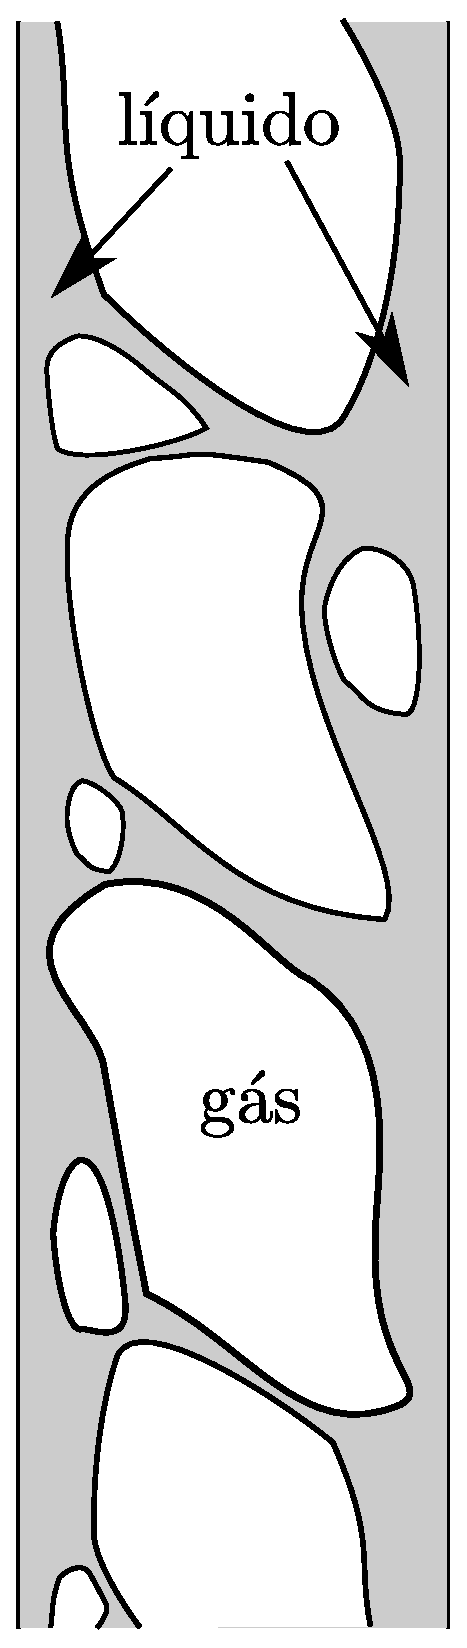
\includegraphics[angle=00, scale=0.3]{v_churn.eps}
		\hspace{0.8cm}}
		\subfloat[Pouco anular]
		{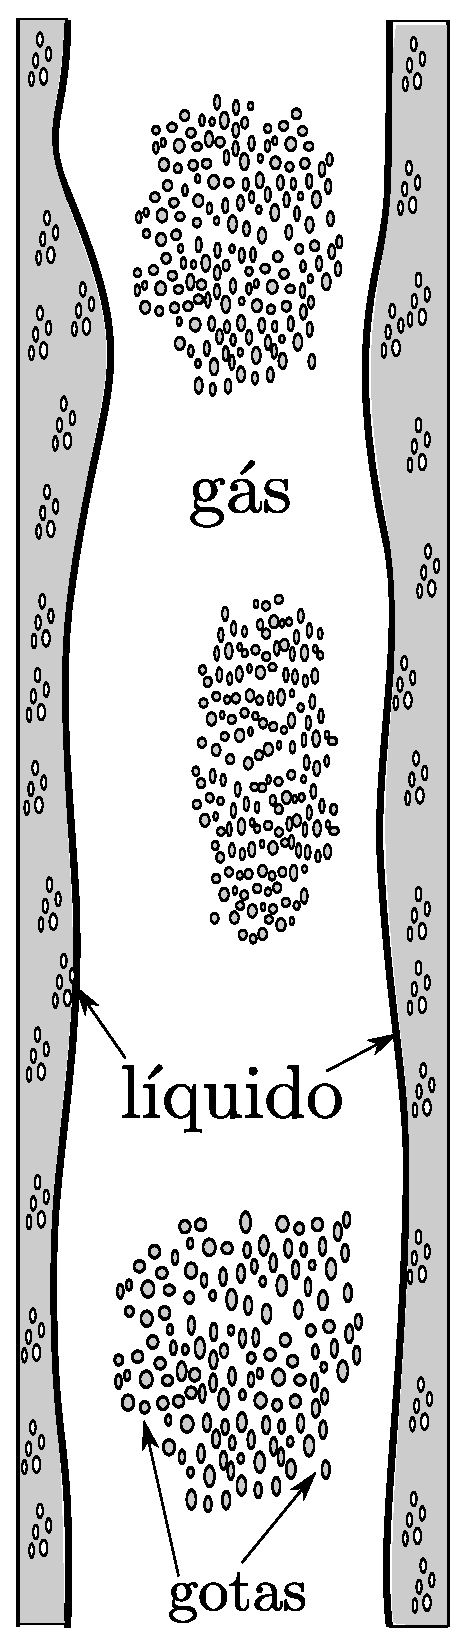
\includegraphics[angle=00, scale=0.3]{v_wispy-annular.eps}
		\hspace{0.8cm}}
		\subfloat[Anular]
		{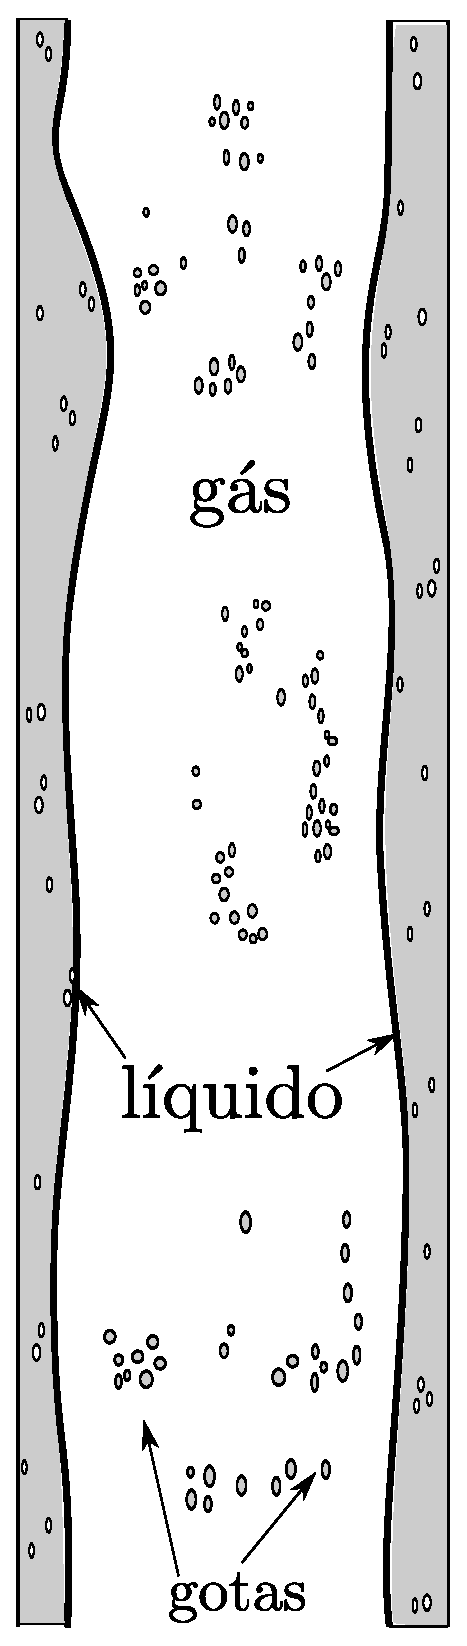
\includegraphics[angle=00, scale=0.3]{v_annular.eps}}
	\end{center}
	\caption[Escoamentos bif\'asicos em tubos verticais.]{Escoamentos
	 bif\'asicos em tubos verticais. Em todos os casos o escoamento se
	 faz de baixo para a cima. Os efeitos gravitacionais s\~ao uniformes
	 ao longo do eixo horizontal, fazendo com que o escoamento apresente
	 alguma estrutura sim\'etrica.} \label{fig:vertical} 
\end{figure}

\begin{itemize}
	\item Bolhas dispersas ou \emph{Bubbly}: no escoamento em
	bolhas, o g\'as ou a fase vapor est\'a distribu\'ida na fase cont\'inua
	l\'iquida como um aglomerado de bolhas. Em uma situa\c c\~ao extrema,
	estas bolhas podem apresentar formato esf\'erico e de pequeno
	di\^ametro ou apresentar formato de corpo alongado com a uma das
	extremidades arredondadas. Neste \'ultimo estado, mesmo n\~ao
	apresentando tamanhos compar\'aveis ao di\^ametro do tubo, o
	padr\~ao das bolhas pode trazer alguma semelhan\c ca ao escoamento
	em golfadas.
	\item Golfadas ou \emph{Slug}: neste tipo de escoamento, as
	bolhas apresentam aproximadamente o mesmo di\^ametro do tubo, com
	isso os efeitos de parede s\~ao mais evidentes. O nariz da bolha tem
	um formato caracter\'istico arredondado devido \`a press\~ao e ao
	escoamento, enquanto que as laterais s\~ao separadas por um filme
	l\`iquido que vai suavemente diminuindo at\'e chegar \`a parte de
	tr\'as da bolha. O termo \emph{slug} representa o l\'iquido que
	separa sucessivas bolhas de g\'as ou vapor. Dependendo do
	escoamento, pequenas bolhas podem ou n\~ao estar presentes entre as
	bolhas principais.
	\item Batido ou \emph{Churn flow}: a interface de largas bolhas 
	de g\'as ou vapor se quebra, formando o escoamento do tipo golfadas
	em uma distribui\c c\~ao ca\'otica. Nele, a fase l\'iquida \'e empurrada
	em dire\c c\~ao \`as paredes do canal. Este escoamento tamb\'em \'e
	conhecido como semi-anular ou golfada-anular, devido ao car\'arter
	transit\'orio deste padr\~ao.
	\item Pouco anular ou \emph{Wispy-annular flow}: o filme l\'iquido
	apresenta grande espessura nas paredes do tubo com uma
	consider\'avel quantidade de l\'iquido arrastada para dentro do
	n\'ucleo de g\'as ou vapor. Este tipo de padr\~ao de escoamento foi
	primeiramente identificado pelo trabalho de \cite{hewitt1970}. Em um
	padr\~ao geral, muitas bolhas s\~ao encontradas no filme l\'iquido
	pr\'oximo \`as parades do tubo, enquanto que grandes gotas s\~ao
	arrastadas dentro do n\'ucleo de g\'as ou vapor. Este padr\~ao de
	escoamento \'e encontrado em grandes vaz\~oes m\'assicas e, devido
	\'a grande quantidade de bolhas no filme l\'iquido, este escoamento
	pode ser confundido com o escoamento em bolhas. 
	\item anular ou \emph{Annular flow}: um filme l\'iquido \'e formado
	pr\'oximo \`as paredes do tubo devido ao aparecimento de um n\'uclo
	cont\'inuo de g\'as ou vapor no meio do tubo. O aparecimento de
	ondas pode ser notado na superf\'icie do filme. Devido a sucessiva
	quebra destas ondas, pode haver a forma\c c\~ao de gotas no n\'ucleo de
	g\'as ou vapor. Diferentemente do escoamento do tipo
	\emph{Wispy-annular}, as gotas est\~ao separadas ao in\'es de
	aglomeradas.
\end{itemize}

\subsection{Escoamentos horizontais}

Os padr\~oes de escoamento comumente encontrados em escoamentos
tubulares horizontais e inclinados s\~ao complexos devido \`a sua
natureza n\~ao sim\'etrica causada pelo influ\^encia do campo
gravitacional. Entretanto s\~ao bem considerados at\'e hoje os padr\~oes
multif\'asicos sugeridos por \cite{alves1954} e apresentados
de forma esquem\'atica na Fig.~(\ref{fig:horizontal}). 

\begin{figure}[h!]
	\begin{center}
% 		\subfloat[]
% 		{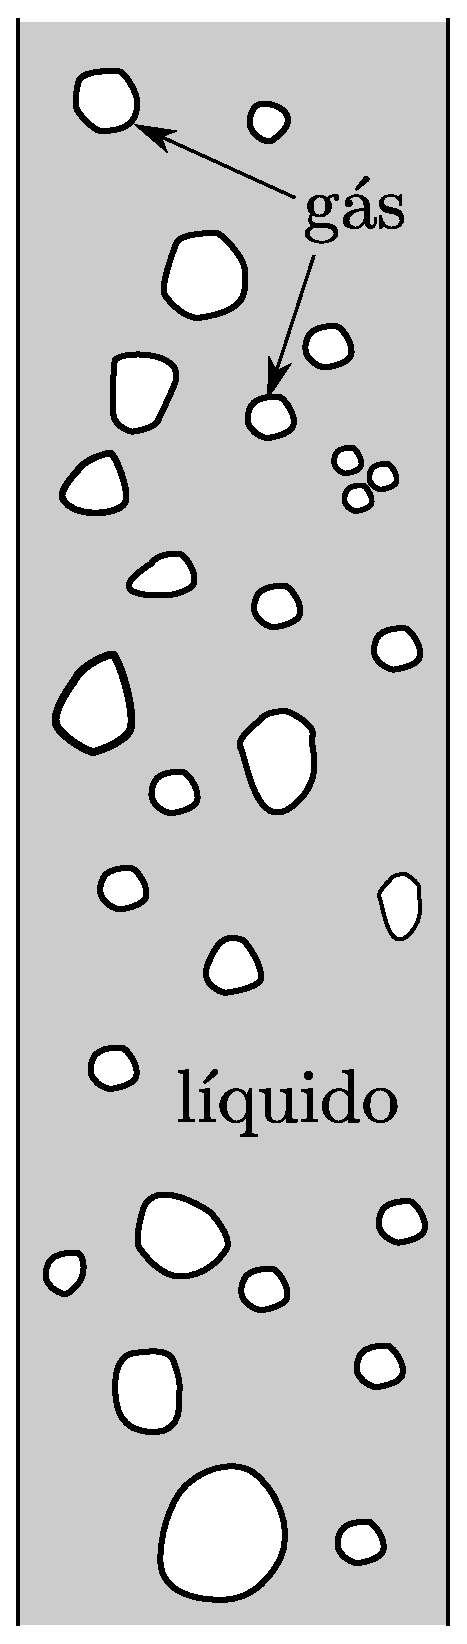
\includegraphics[angle=00, scale=0.3]{v_bubbly.eps}
% 		\hspace{0.8cm}}
		\subfloat[Bolhas dispersas]
		{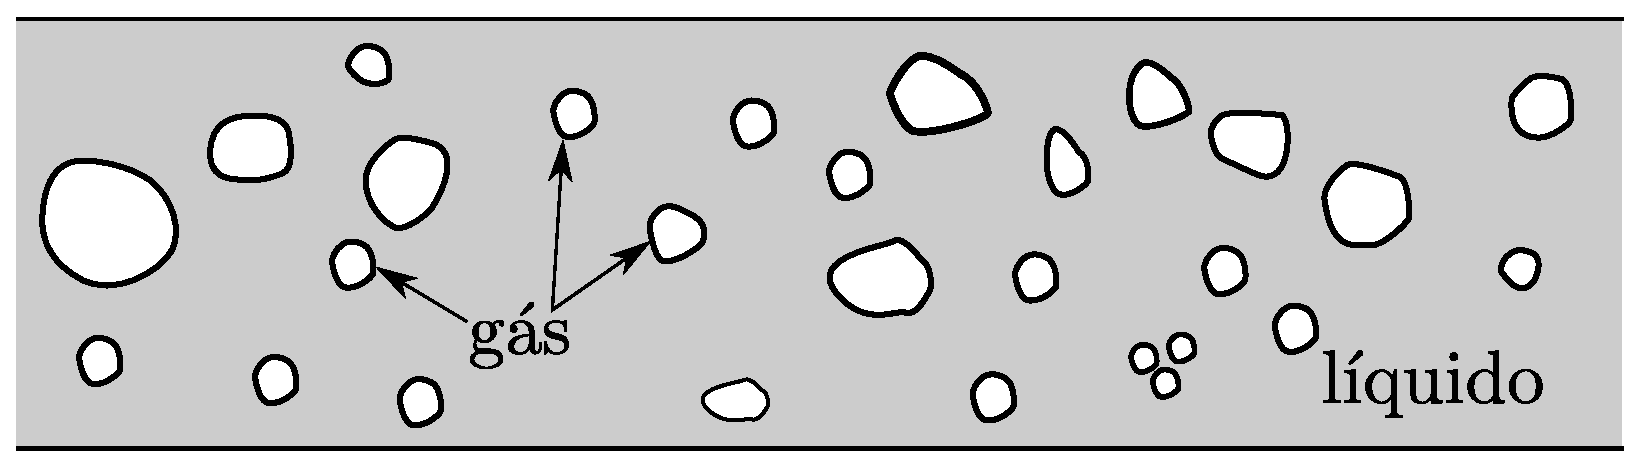
\includegraphics[angle=00, scale=0.265]{h_bubbly.eps}
 		\hspace{0.2cm}}
		\subfloat[Bolhas]
		{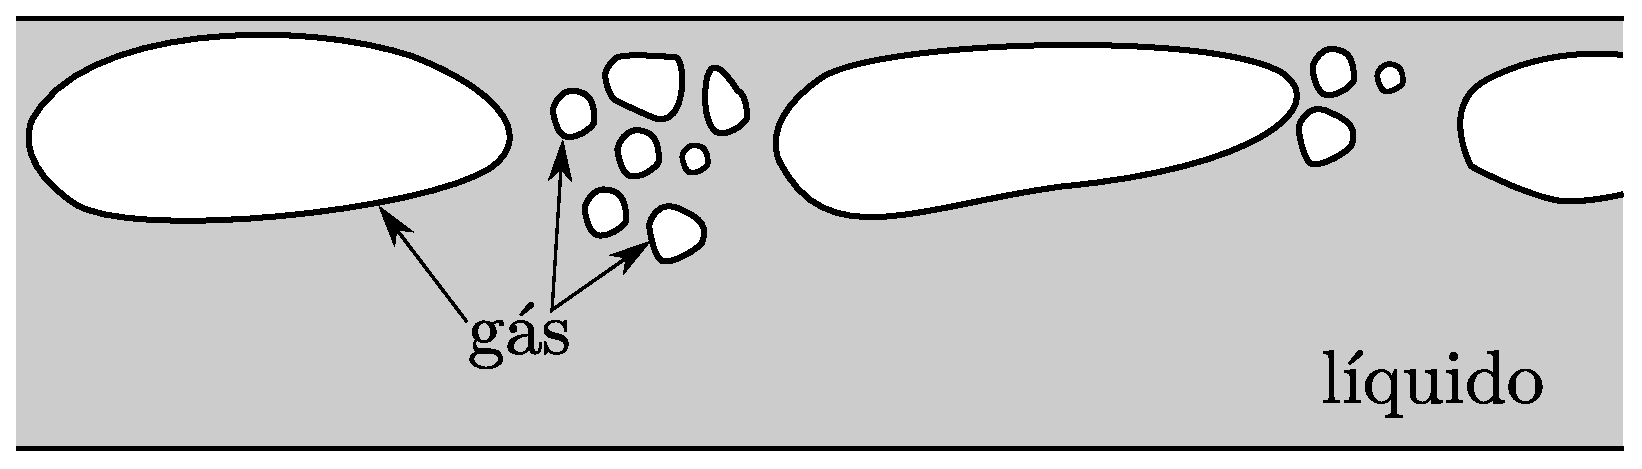
\includegraphics[angle=00, scale=0.265]{h_plug.eps}}\\
		\subfloat[Golfadas]
		{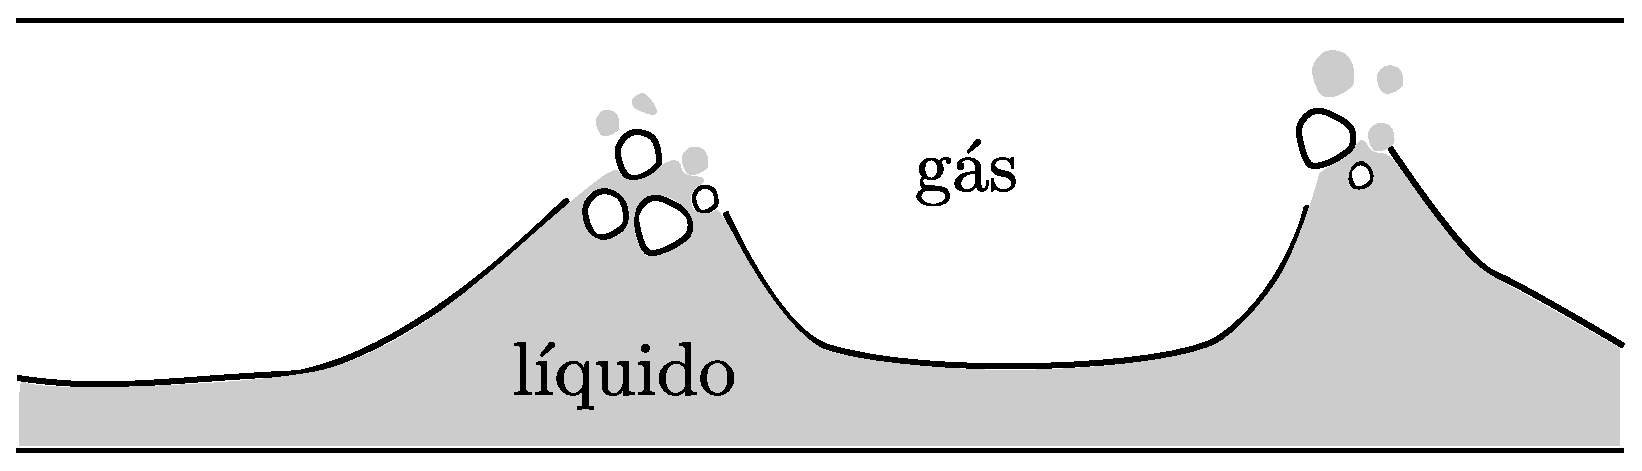
\includegraphics[angle=00, scale=0.265]{h_slug.eps}
 		\hspace{0.2cm}}
		\subfloat[Estratificado]
		{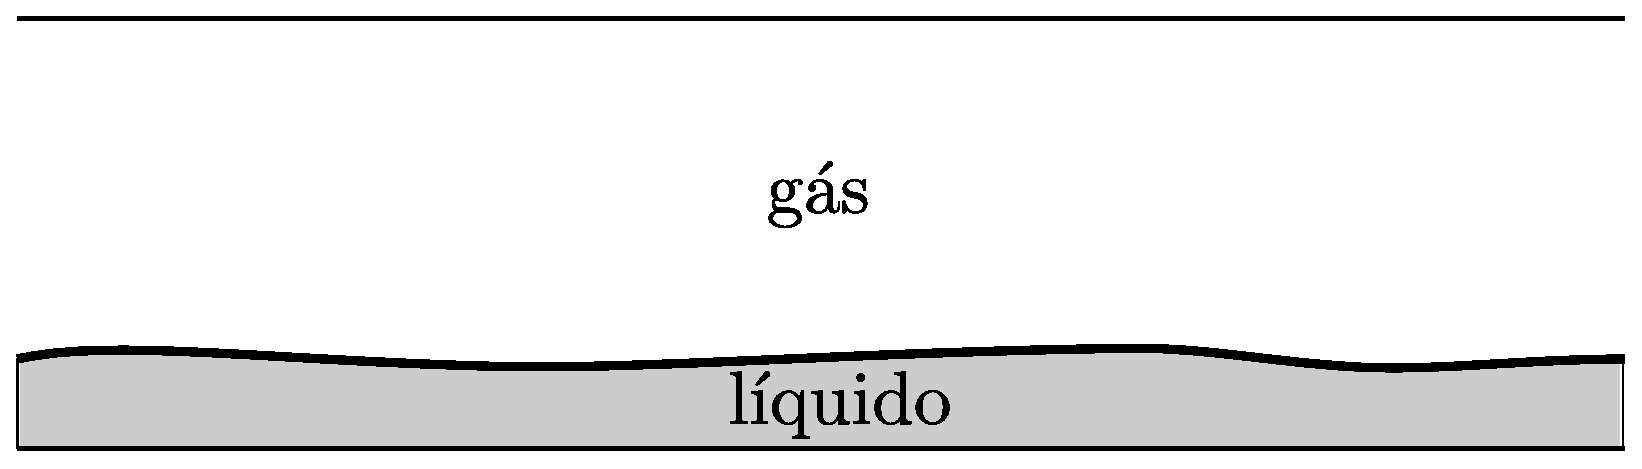
\includegraphics[angle=00, scale=0.265]{h_stratified.eps}}\\
		\subfloat[Estratificado ondulado]
		{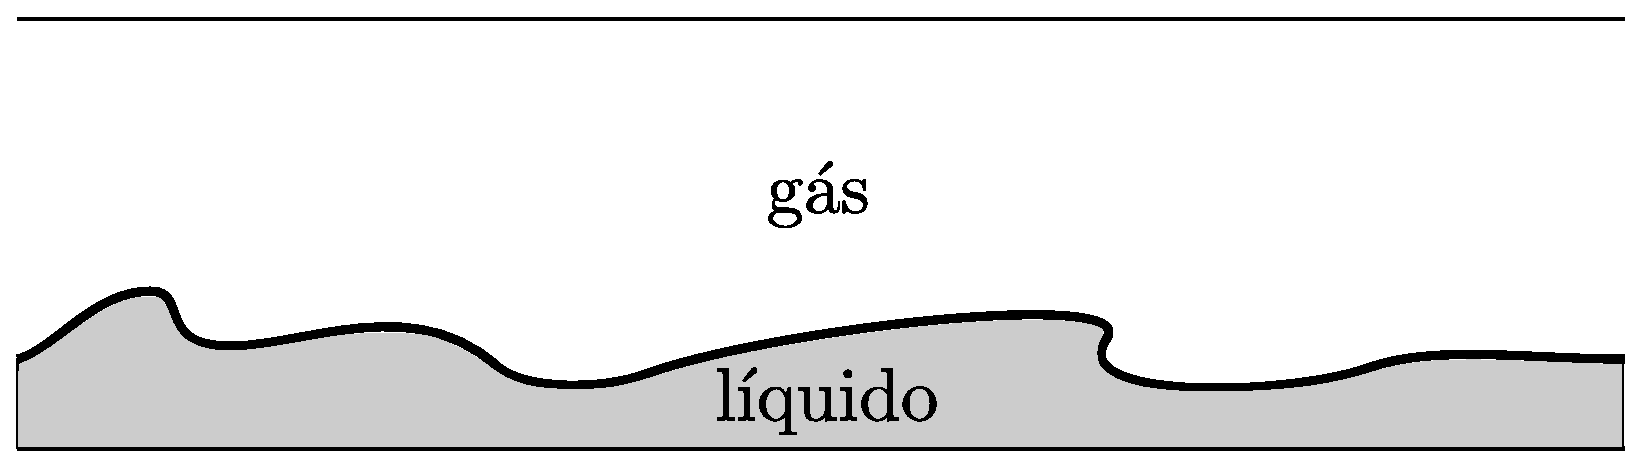
\includegraphics[angle=00, scale=0.265]{h_wavy.eps}
 		\hspace{0.2cm}}
		\subfloat[Anular]
		{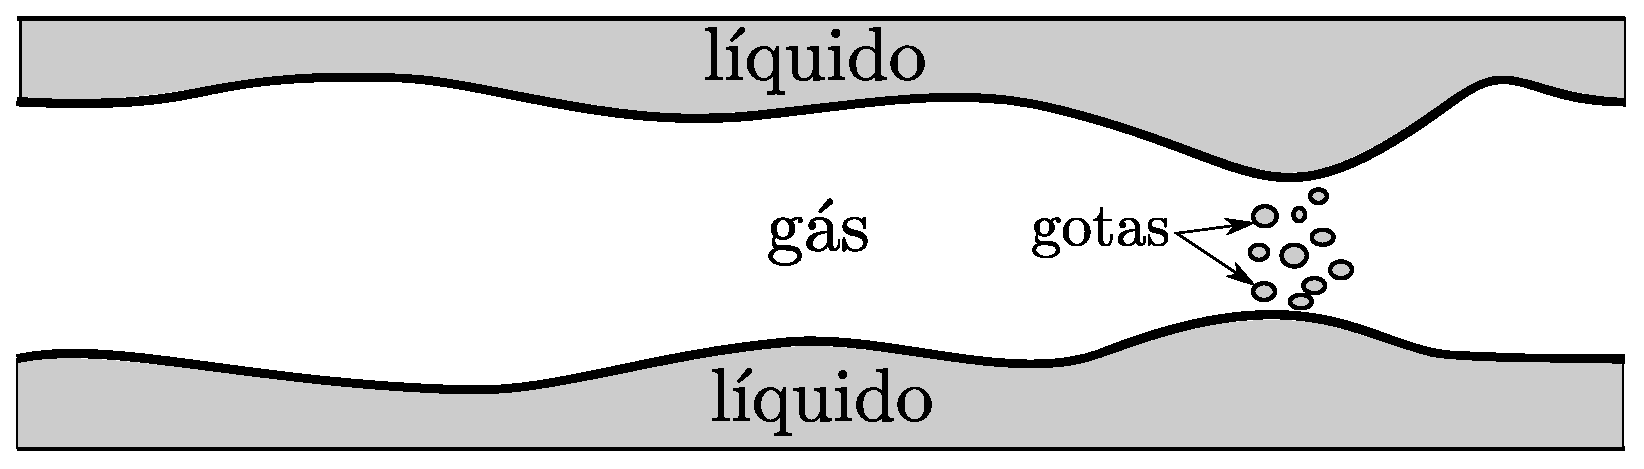
\includegraphics[angle=00, scale=0.265]{h_annular.eps}}
	\end{center}
	\caption[Escoamentos bif\'asicos em tubos horizontais.]{Escoamentos
	 bif\'asicos em tubos horizontais. Em todos os casos o escoamento se
	 faz da esquerda para a direta. Dependendo da velocidade de entrada
	 das fases, um padr\~ao pode ser identificado. Como pode ser
	 verificado pela posi\c c\~ao das bolhas, a gravidade exerce uma
	 influ\^encia imediata nas fases, uma vez que o fluido menos denso
	 tende a se movimentar na parte de cima do tubo.}
  \label{fig:horizontal} 
\end{figure}

\begin{itemize}
	\item Bolhas dispersas ou \emph{Bubbly}: este escoamento \'e
	similar ao apresentado anteriormente para escoamento vertical, com a
	diferen\c ca que as bolhas de g\`as ou vapor tendem a se movimentar
	na metade superior do tubo. Fato justificado pela menor densidade da
	bolha comparada ao l\'iquido. Em uma velocidade moderada de ambas as
	fases presente no escoamento, a distribui\c c\~ao de bolhas \'e uniforme
	ao longo do tubo, enquanto que para velocidades mais elevadas o
	padr\~ao de escoamento se assemelha ao \emph{Wispy-annular}.
	\item Bolhas \emph{Plug}: escoamento similar ao do tipo golfadas em
	tubos verticais. Como no caso de bolhas dispersas, a bolhas de g\'as
	ou vapor tendem a atravessar o tubo na metade superior, devido ao
	campo gravitacional.
	\item Estratificado ou \emph{Stratified}: escoamento separado por
	uma interface suave, onde geralmente \'e encontrado em baixas
	velocidades das fases l\'iquida e gasosa.
	\item Estratificado ondulado ou \emph{Wavy}: as ondas s\~ao formadas
	quando a velocidade na fase gasosa \'e aumentada. Estas ondas se
	movimentam na direc\~ao do escoamento.  
	\item golfada ou \emph{Slug}: com o aumento da velocidade da fase
	de vapor, a amplitude das ondas tamb\'em aumenta, se aproximando da
	parede do tubo. A parte superior do tubo atr\'as da onda \'e molhada
	por um filme l\'iquido que \'e drenado para o meio da fase
	l\'iquido.
	\item Anular ou \emph{Annular}: a vaz\~ao da fase gasosa \'e t\~ao
	alta que \'e capaz de sustentar a fase l\'iquida pr\'oxima \`a
	parede do tubo, originando um n\'ucleo de g\'as ou vapor. Em sua
	se\c c\~ao transversal, o l\'iquido pode n\~ao ser cont\'inuo ao redor
	de toda a circunfer\^ncia, po\'em ser\'a mais espessa na base do
	tubo.
\end{itemize}

\subsection{Mapa de padr\~oes de escoamentos}
Os mapas de padr\~oes de escoamento s\~ao utilizados para a
identifica\c c\~ao do tipo de escoamento (golfadas, anular, estratificado
etc.) atrav\'es de par\^ametros conhecidos como vaz\~ao m\'assica,
fra\c c\~ao de vazios, qualidade de vapor etc. Estes mapas existem para
diferentes tipos de fluidos, dimens\~ao de tubos, graus de mistura e
muitos outros. Basicamente, eles podem ser divididos em duas classes:
adiab\'aticos e diab\'aticos. O primeiro \'e usualmente utilizado para
escoamentos do tipo ar/\'agua, enquanto o segundo pode ser encontrado em
refrigerantes em evapora\c c\~ao. 

Os mapas de padr\~oes s\~ao representados como \'areas em gr\'aficos, em
fun\c c\~ao das velocidades superficiais ou qualquer outro par\^ametro geral
que contenha tal defini\c c\~ao . \'E importante notar que o padr\~ao de
escoamento \'e tamb\'em influenciado por outros tipos de par\^ametros,
por\'em sua descri\c c\~ao atrav\'es de gr\'aficos bi-dimensionais. Na
literatura, muitos mapas podem ser encontrados para diferentes fluidos e
em diferentes condi\c c\~oes. O leitor interessado poder\'a consultar
algumas refer\^encias cl\'assicas como (\cite{collier1996},
\cite{whalley1987} e \cite{thome2008}).

A Fig.~(\ref{fig:map}a) representa um mapa de padr\~oes de escoamento
para ar/\'agua, em condi\c c\~oes de press\~ao atmosf\'erica, para
canais verticais (\cite{hewitt1969}). Neste mapa pode-se observar que
cada padr\~ao de escoamento ocupa uma \'area no gr'afico e as linhas
tracejadas delimitam a transi\c c\~ao.  Como pode-se observar tamb\'em,
estas mesmas linhas n\~ao ocupam todo o limite do gr\'afico, o que
sugere a falta de dados experimentais para descrever as transi\c c\~oes
em toda a escala. \'E importante notar que estes mapas devem ser
observados n\~ao mais do que um guia grosseiro de padr\~oes de
escoamentos, pois os fluxos de quantidade de movimento por si s\'o n\~ao
s\~ao capazes de representar com exatid\~ao a influ\^encia das
propriedades f\'isicas do fluido nem o di\^ametro do tubo.

A Fig.~(\ref{fig:map}b) descreve um outro mapa de padr\~oes, por\'em
para escoamento horizontal (\cite{baker1954}). Este mapa \'e largamente
utilizado na ind\'ustria petroqu\'imica. No mapa pode-se identificar os
padr\~oes de escoamento em diferentes velocidades m\'assicas
superficiais ($G_f$ e $G_g$). 

\begin{figure}[ht!]
	\subfloat[]
	{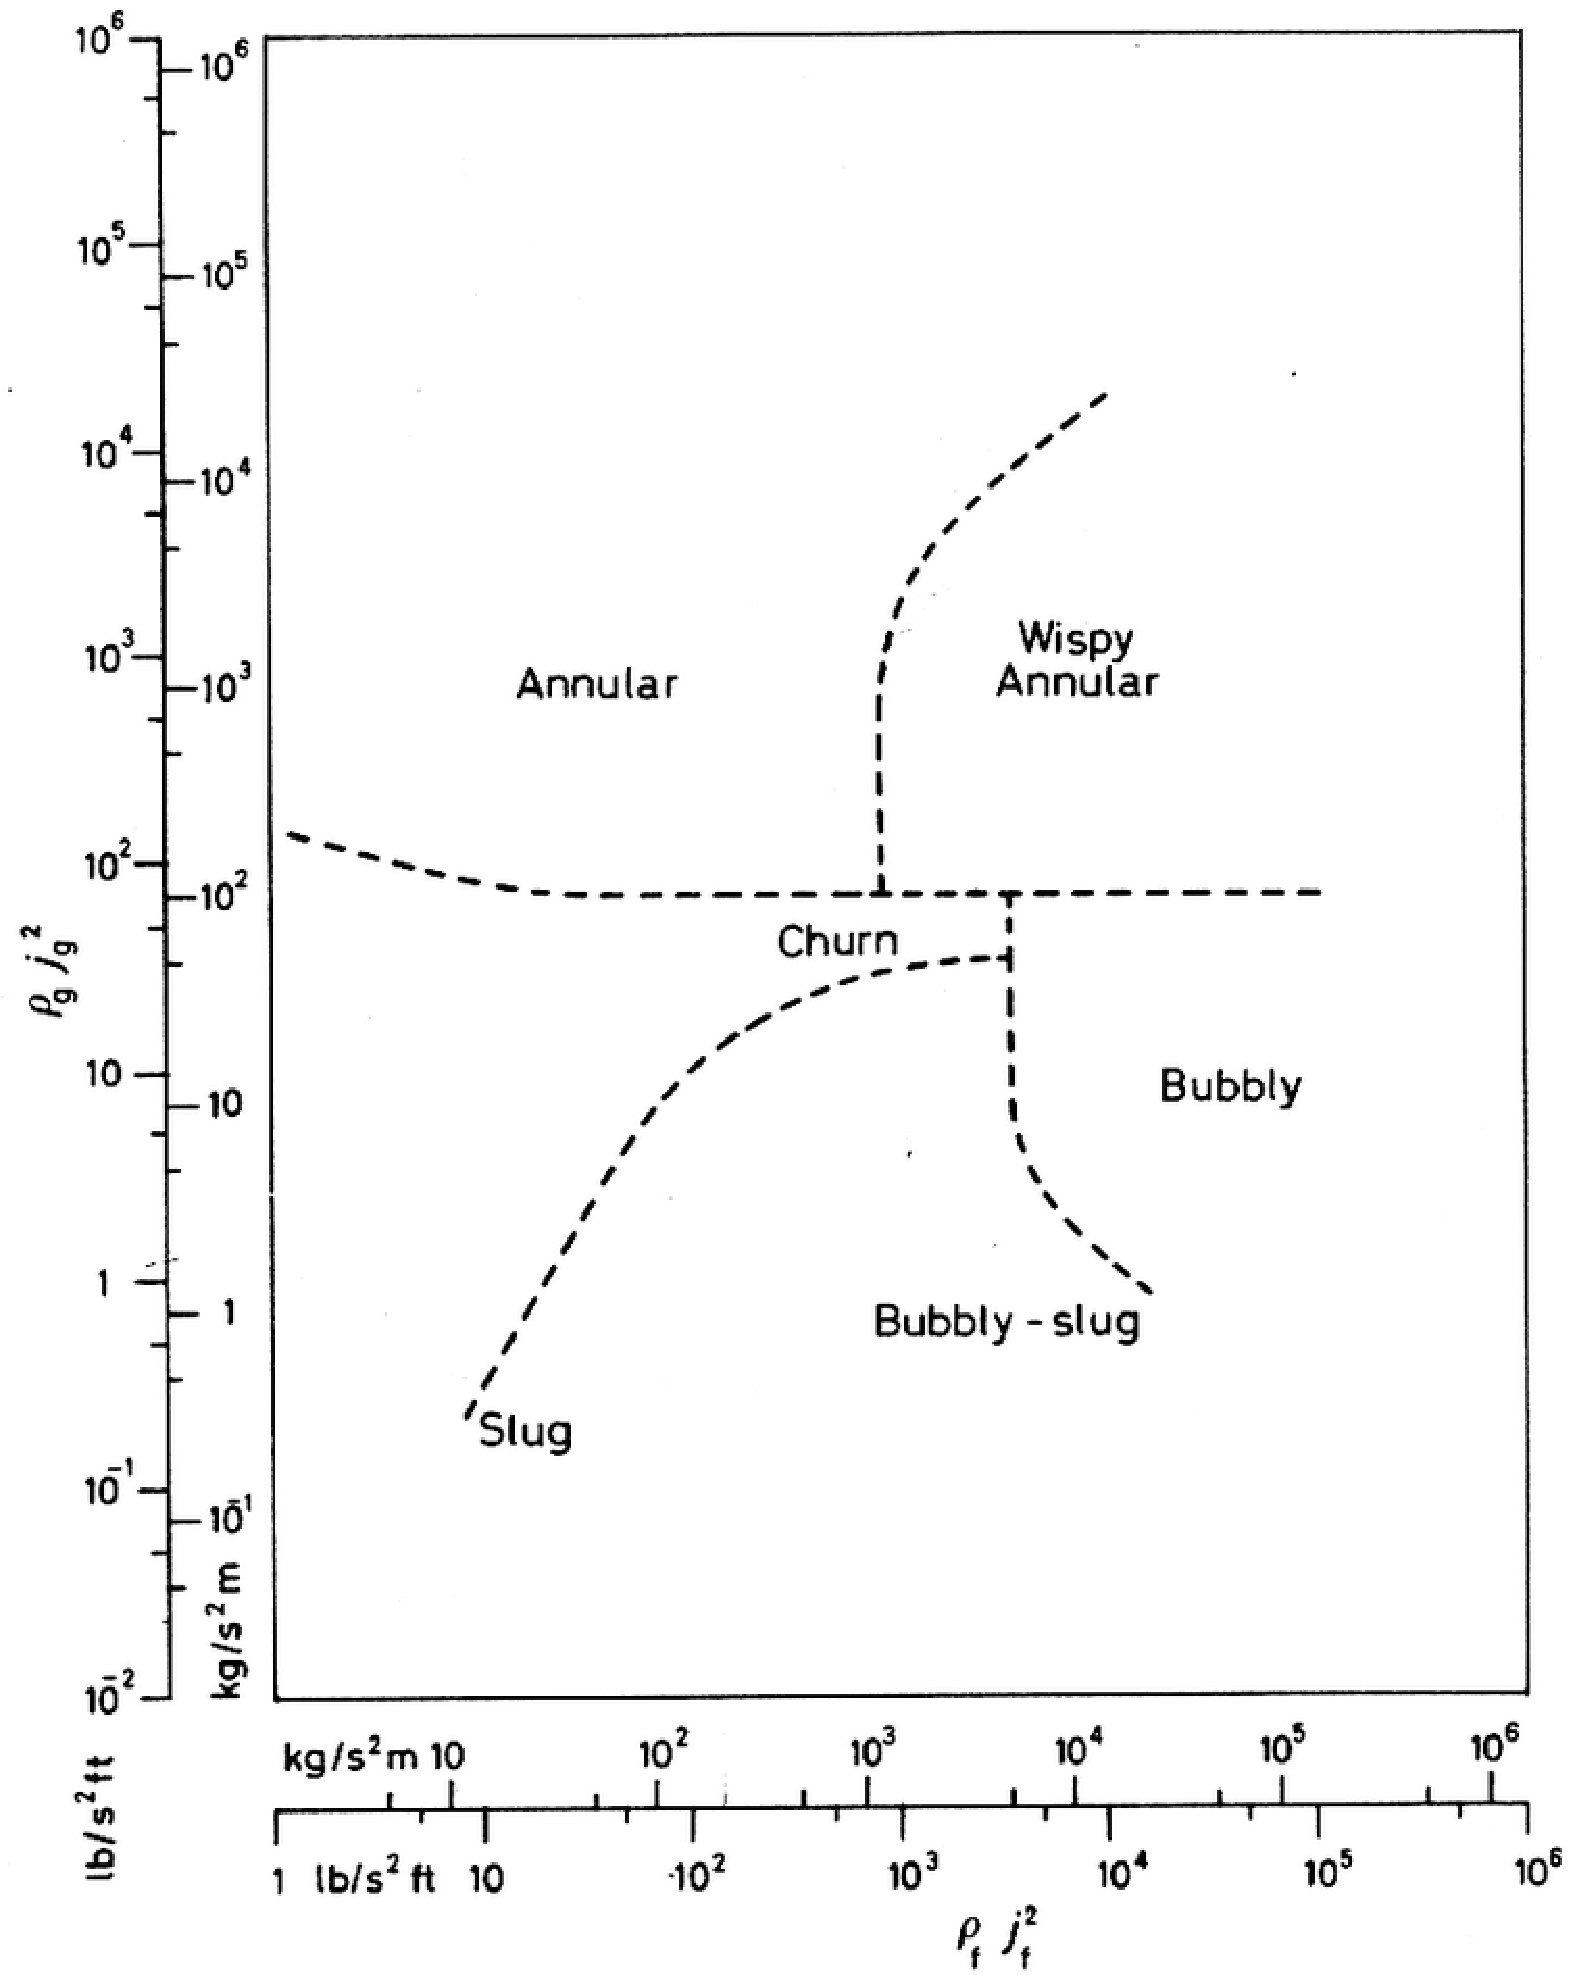
\includegraphics[scale=0.27,angle=-0.5]{hewitt1969.eps}}
	\hspace{0.2cm}
	\subfloat[]
	{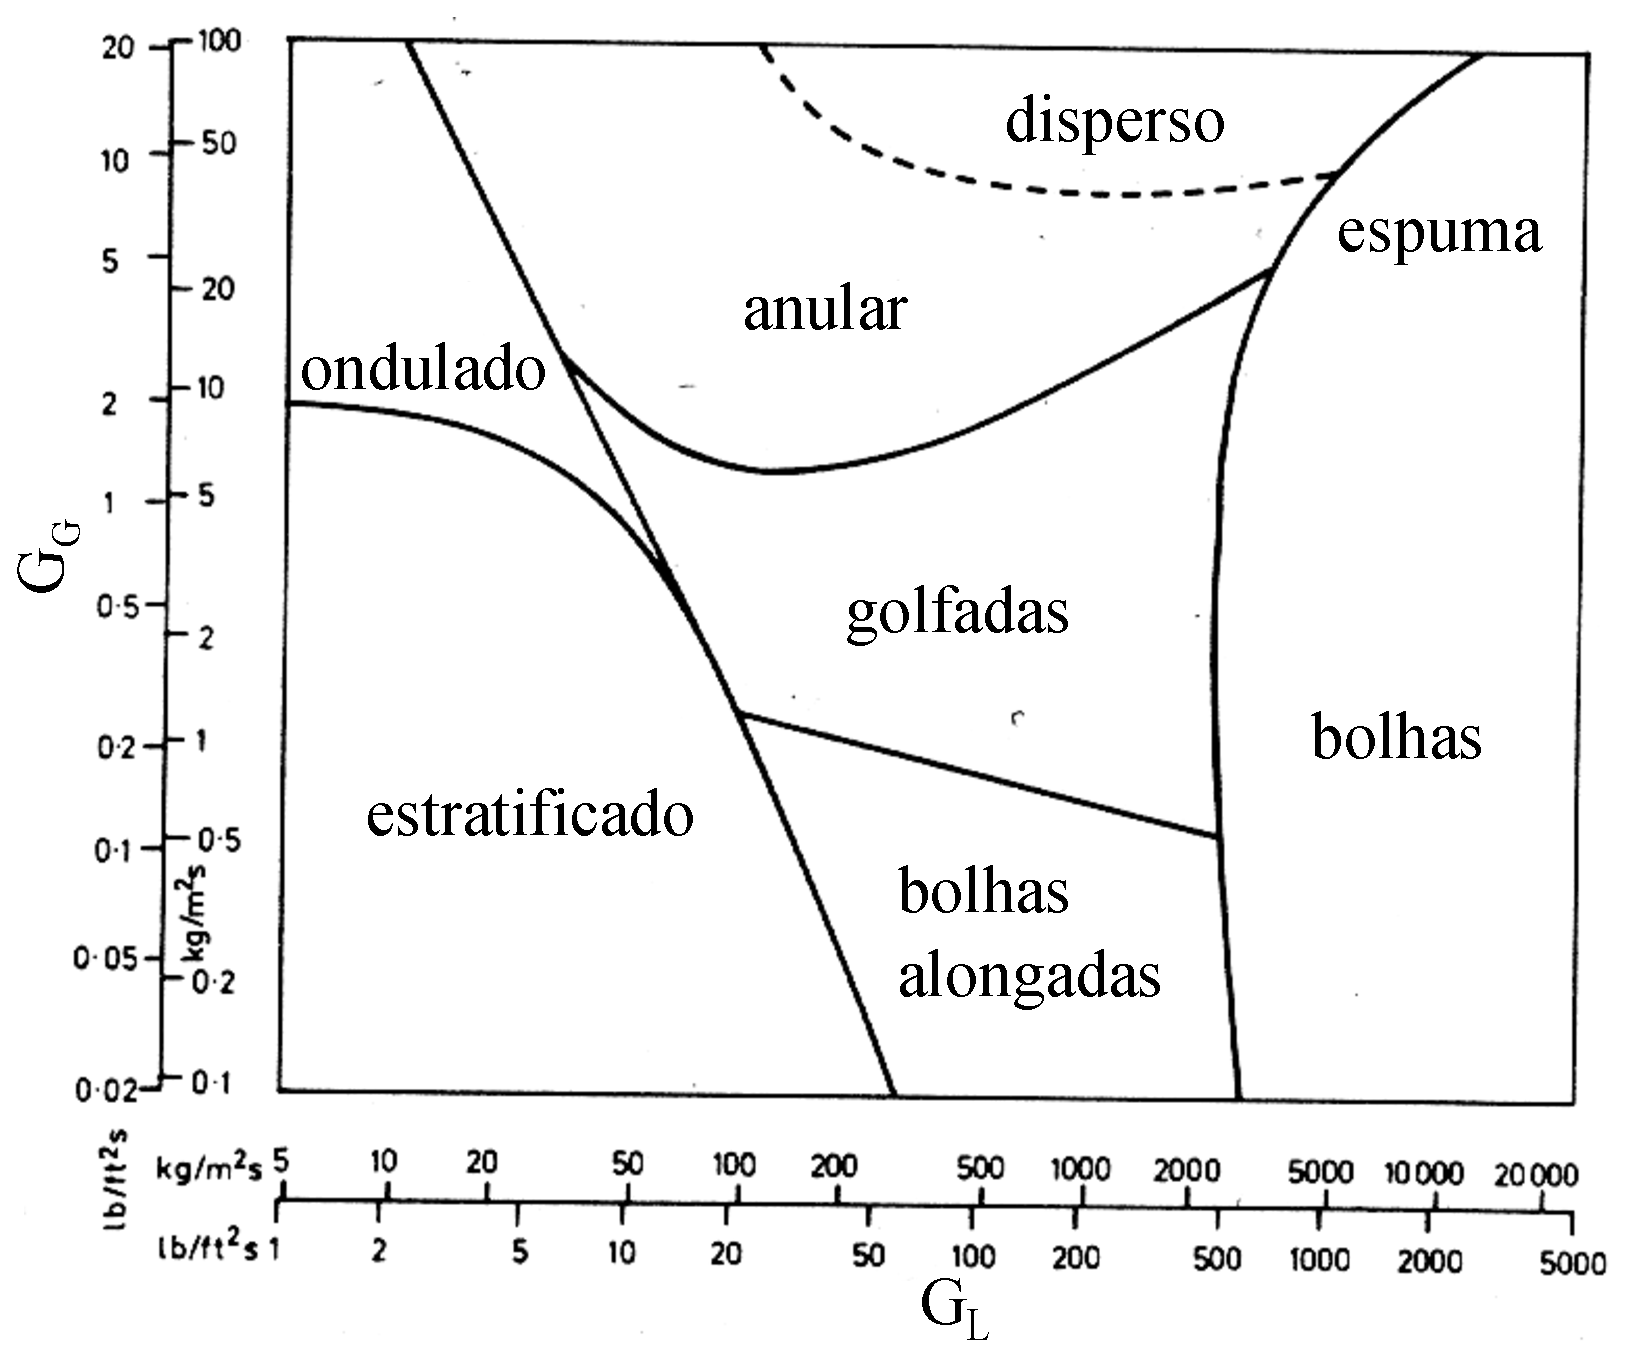
\includegraphics[scale=0.27,angle=1]{baker1954.eps}}
	\caption[Mapas de padr\~oes de escoamento bif\'asico.]{Mapas de
	 padr\~oes de escoamento bif\'asico. As linhas cont\'inuas e
	 tracejadas representam a transi\c c\~ao dos padr\~oes de
	 escoamento. (a) Escoamento vertical para ar/\'agua
	 (\cite{hewitt1969}). (b) Escoamento horizontal para ar/\'agua
	 (\cite{baker1954}).}
	\label{fig:map} 
\end{figure}

\section{Problemas}

1) Descreva a diferen\c ca entre referencial \emph{Euleriano} e
\emph{Lagrangiano}.

2) Mostre as diferen\c ca entre escoamentos em bolhas e golfadas para
tubos verticais.

3) Por que em escoamentos horizontais do tipo Bolhas dispersas, a bolhas
tendem a se locomover na metade superior do tubo? Qual o par\^ametro
adimensional que caracteriza este fen\^omeno?

4) Para que servem os mapas de padr\~oes de escoamento e como s\~ao
classificados?

\bibliographystyle{plain}
\bibliography{refANJOS}

\end{document}

\typeout{ *************** End of file main.tex *************** }
